%\documentclass[10pt,twocolumn]{article}
%\documentclass[pageno]{jpaper}
%\documentclass{sig-alternate}
\documentclass[sigplan,10pt,anonymous,nocopyrightspace]{acmart}\settopmatter{printfolios=true}
\usepackage{mathptmx} % This is Times font

%\newcommand{\asplossubmissionnumber}{209}
%\newcommand{\iscasubmissionnumber}{457}
\setcopyright{none}             %% For review submission



%\usepackage{times}
\usepackage{fullpage}
\usepackage[utf8]{inputenc}
\usepackage[english]{babel}
\usepackage{amstext,amssymb,amsmath,amsthm}
\usepackage{verbatim}
\usepackage{subfigure}
\usepackage{color}
\usepackage{paralist}
\usepackage{multirow}
\usepackage{listings}
\usepackage{array}
\usepackage{graphicx,color}
\usepackage{moreverb}
\usepackage{xspace}
\usepackage{algorithmic}
\usepackage{algorithm}
\usepackage{times}
\usepackage{relsize}
\newcolumntype{x}[1]{>{\centering\arraybackslash}p{#1}}
\newlength\SUBSIZE
\newcommand{\ONECOLFIGMUL}{0.81}
\newcommand{\TALLFIGMUL}{0.75}
\newcommand{\ie}{\textit{i.e.},~}
\newcommand{\eg}{\textit{e.g.},~}
\usepackage{caption}
%\usepackage{subcaption}

\newcounter{cnt}
% \def\full{0}
\newtheorem{lem}[cnt]{Lemma}
\newtheorem{thm}[cnt]{Theorem}
\newtheorem{problem}[cnt]{Problem}
\newtheorem{defn}[cnt]{Definition}
\newtheorem{fact}[cnt]{Fact}
\newtheorem{example}[cnt]{Example}
\newtheorem{corollary}[cnt]{Corollary}
\newtheorem{assumption}[cnt]{Assumption}
\newtheorem{claim}[cnt]{Claim}
\newcommand{\ip}[2]{\langle #1,#2\rangle}
\renewcommand{\algorithmicrequire}{\textbf{Input:}}
\renewcommand{\algorithmicensure}{\textbf{Output:}}
\newcommand{\nptheta}{\hat\theta}
\newcommand{\symdiff}{\Delta}
\newcommand{\noise}{{\sf Noise}}
\newcommand{\privtheta}{\theta_{priv}}
\renewcommand{\paragraph}[1]{\vspace{3pt}\noindent\textbf{#1}}
\newcommand{\scrX}{\ensuremath{\mathcal{X}}}
\newcommand{\scrZ}{\ensuremath{\mathcal{Z}}}
\newcommand{\rA}{\ensuremath{\rightarrow}}
\newcommand{\rrA}{\ensuremath{\longrightarrow}}
\newcommand{\qB}{\ensuremath{\mathbf{q}}}
\newcommand{\XB}{\ensuremath{\mathbf{X}}}
\newcommand{\zeroB}{\ensuremath{\mathbf{0}}}
\newcommand{\sm}{\mbox{\textendash}}
\newcommand{\ltwo}[1]{\left\|#1\right\|_2}
\newcommand{\lone}[1]{\left\|#1\right\|_1}
\newcommand{\eps}{\epsilon}
\newcommand{\A}{\mathcal{A}}
\newcommand{\D}{\mathcal{D}}
\newcommand{\T}{\mathcal{T}}
\newcommand{\R}{\mathbb{R}}
\newcommand{\K}{\mathcal{K}}
\newcommand{\mineig}{\eta}
\newcommand{\I}{\mathbb{I}}
\newcommand{\E}{\mathbb{E}}
\newcommand{\F}{\mathcal{C}}
\newcommand{\hatw}{\hat{w}}
\newcommand{\hatv}{{\hat{v}}}
\newcommand{\hatV}{{\hat{V}}}
\newcommand{\hatW}{{\hat{W}}}
\newcommand{\kl}{{\sf KL}}
\newcommand{\dagw}{w^\dagger}
\newcommand{\tildew}{\tilde{w}}
\newcommand{\tildeF}{\tilde{F}}
\newcommand{\tildef}{\tilde{f}}
\newcommand{\re}{\mathbb{R}}
\newcommand{\B}{\mathbb{B}}
\newcommand{\bP}{\mathbb{P}}
\renewcommand{\P}{\mathcal{P}}
\newcommand{\grad}{\bigtriangledown}
\newcommand{\mypar}[1]{\smallskip
\noindent{\bf\em {#1}.}}
\newcommand{\etal}{\emph{et al.}}
\newcommand{\negl}{\text{negl}}
\newcommand{\mynote}[3]{\marginpar{\parbox{0.7in}{\tiny {\color{#2} {\sc #1}: {\sf #3}}}}}
\newcommand{\atnote}[1]{\mynote{at}{blue}{#1}}
\newcommand{\nmnote}[1]{\mynote{prmohan}{red}{#1}}
\newcommand{\ignore}[1]{}
\newcommand{\rpm}{\sbox0{$1$}\sbox2{$\scriptstyle\pm$}  \raise\dimexpr(\ht0-\ht2)/2\relax\box2 }
\newcommand{\TODO}[1]{{\bf TODO: #1}}
\newcommand{\NOTE}[1]{{\bf NOTE: #1}}

\newcommand{\name}{\textsc{GUPT}\xspace}
\newcommand{\nameplain}{GUPT\xspace}
\newcommand{\aname}{a \textsc{GUPT}\xspace}
\newcommand{\Aname}{A \textsc{GUPT}\xspace}
\newcommand{\C}{\mathcal{C}}
\newcommand{\hatd}{{\hat d}}
\newcommand{\hatf}{{\hat f}}
\newcommand{\tr}{{\sf tr}}
\newcommand{\Lap}{\mathsf{Lap}}
\newcommand{\M}{\mathcal{M}}
\newcommand{\besta}{a_{{\sf best}}}
\newcommand{\Vect}{\text{vec}}
\newcommand{\Vech}{\text{vech}}
\newcommand{\rank}{\text{rank}}
\newcommand{\diag}{\text{diag}}
\newcommand{\nnz}{\text{nnz}}
\newcommand{\y}{\mathbf{y}}
\newcommand{\w}{\mathbf{w}}
\newcommand{\x}{\mathbf{x}}
\newcommand{\z}{\mathbf{z}}
\DeclareMathOperator*{\argmin}{arg\,min}
\DeclareMathOperator*{\argmax}{arg\,max}

\usepackage{balance}
%\usepackage{times}
%\usepackage{fullpage}
\usepackage{enumitem}
%\usepackage[shortlabels]{enumitem}
%\usepackage{mathtools}
\usepackage[normalem]{ulem}
\usepackage{todonotes}
\usepackage{subfig}
\usepackage{mathtools}
\usepackage{algorithm2e}
\usepackage{algorithmic}
\usepackage{wrapfig}
%\usepackage{algorithmicx}
%\usepackage{algpseudocode}

%\newtheorem{theorem}{Theorem}
%\usepackage{amstext,amssymb,amsmath,amsthm}
%\DeclarePairedDelimiter{\ceil}{\lceil}{\rceil}
%\DeclarePairedDelimiter\floor{\lfloor}{\rfloor}
\let\bibhang\relax
\let\citename\relax
\let\bibfont\relax
\let\Citeauthor\relax
\let\citet\relax
\let\citep\relax
\let\citealt\relax
\let\citealp\relax
\let\Citet\relax
\let\Citep\relax
\let\Citealt\relax
\let\Citealp\relax
\let\citefullauthor\relax
\let\citetext\relax
\let\defcitealias\relax
\expandafter\let\csname ver@natbib.sty\endcsname\relax
\usepackage[natbib=true,backend=bibtex,firstinits=true,style=numeric-comp,sorting=nyt,defernumbers,maxnames=99,maxcitenames=99]{biblatex}

\setlist{noitemsep,topsep=0pt}

%\setlength{\itemsep}{0pt}
%\setlength{\textheight}{9.0in}
%\setlength{\columnsep}{0.25in}
%\setlength{\textwidth}{6.50in}
%\setlength{\topmargin}{0.0in}
%\setlength{\headheight}{0.0in}
%\setlength{\headsep}{0.0in}
\setlength{\leftmargini}{0em}%
\setlength{\leftmarginii}{1em}%

\setlength{\abovecaptionskip}{1pt plus 2pt minus 2pt}
\setlength{\floatsep}{3pt}
\setlength{\intextsep}{4pt}


%--------
\definecolor{mygreen}{rgb}{0,0.6,0}
\definecolor{mygray}{rgb}{0.5,0.5,0.5}
\definecolor{mymauve}{rgb}{0.58,0,0.82}

\definecolor{on}{RGB}{159, 169,133} 
\definecolor{off}{RGB}{255,165,0}%{240,232,205} 
\definecolor{leo}{RGB}{72,181,163} 
\definecolor{poet}{RGB}{249,140,182} 
\definecolor{calnp}{RGB}{117,137,191}
\definecolor{cal}{RGB}{51,255,51} %green


\definecolor{OPTIMAL}{RGB}{0,0,0}
\definecolor{RACE}{RGB}{251,128,114}
\definecolor{CONTROL}{RGB}{255,237,111}
\definecolor{ONLINE}{RGB}{253,180,98}
\definecolor{OFFLINE}{RGB}{252,205,229}
\definecolor{NETFLIX}{RGB}{217,217,217}
\definecolor{HBM}{RGB}{190,186,218}
\definecolor{POET}{RGB}{188,128,189}
\definecolor{CALOREE-NP}{RGB}{179,222,105}
\definecolor{CALOREE-ONLINE}{RGB}{204,235,197}
\definecolor{CALOREE-NETFLIX}{RGB}{141,211,199}
\definecolor{CALOREE-HBM}{RGB}{128,177,211}
\definecolor{PID-CONTROL}{RGB}{255,237,111}
\definecolor{NUCLEAR}{RGB}{190,186,218}
\definecolor{ADAPT-CONTROL}{RGB}{188,128,189}
\definecolor{ONLINE-ADAPT}{RGB}{204,235,197}
\definecolor{NUCLEAR-ADAPT}{RGB}{141,211,199}
\definecolor{HBM-ADAPT}{RGB}{128,177,211}

\usepackage{listings}
\lstset{ %
  backgroundcolor=\color{white},   % choose the background color; you must add \usepackage{color} or \usepackage{xcolor}
  basicstyle=\scriptsize\ttfamily, % the size of the fonts that are used for the code
  breakatwhitespace=false,         % sets if automatic breaks should only happen at whitespace
  breaklines=true,                 % sets automatic line breaking
  captionpos=b,                    % sets the caption-position to bottom
  commentstyle=\color{mygreen},    % comment style
  deletekeywords={...},            % if you want to delete keywords from the given language
  escapeinside={\%*}{*},          % if you want to add LaTeX within your code
  extendedchars=true,              % lets you use non-ASCII characters; for 8-bits encodings only, does not work with UTF-8
  frame=leftline,                  % adds a frame around the code
  keepspaces=true,                 % keeps spaces in text, useful for keeping indentation of code (possibly needs columns=flexible)
  keywordstyle=\color{blue},       % keyword style
  morekeywords={*,...},            % if you want to add more keywords to the set
  numbers=left,                    % where to put the line-numbers; possible values are (none, left, right)
  numbersep=5pt,                   % how far the line-numbers are from the code
  numberstyle=\tiny\color{mygray}, % the style that is used for the line-numbers
  rulecolor=\color{black},         % if not set, the frame-color may be changed on line-breaks within not-black text (e.g. comments (green here))
  showspaces=false,                % show spaces everywhere adding particular underscores; it overrides 'showstringspaces'
  showstringspaces=false,          % underline spaces within strings only
  showtabs=false,                  % show tabs within strings adding particular underscores
  stepnumber=1,                    % the step between two line-numbers. If it's 1, each line will be numbered
  stringstyle=\color{black},     % string literal style
  tabsize=1,                       % sets default tabsize to 2 spaces
  title=\lstname                   % show the filename of files included with \lstinputlisting; also try caption instead of title
}

\usepackage{pgfplots, pgfplotstable}
% options for pgfplots
\pgfplotscreateplotcyclelist{colorbrewer-ylgnbu}{
{fill=on, draw=black},
{fill=off, draw=black},
{fill=leo, draw=black},
{fill=poet, draw=black},
{fill=calnp, draw=black},
{fill=cal, draw=black},
}
\pgfplotsset{compat=1.8,compat/show suggested version=false}
\usetikzlibrary{calc,trees,arrows,patterns,plotmarks,shapes,snakes,er,3d,automata,backgrounds,topaths,decorations.pathmorphing,decorations.markings}
%\pgfplotsset{compat=newest}
\pgfplotsset{
   /pgfplots/bar  cycle  list/.style={/pgfplots/cycle  list={%
        {black,fill=black!30!white,mark=none},%
        {black,fill=red!30!white,mark=none},%
        {black,fill=green!30!white,mark=none},%
        {black,fill=yellow!30!white,mark=none},%
        {black,fill=brown!30!white,mark=none},%
     }
   },
}
% begin of externalization
\usetikzlibrary{external}
\tikzexternalize[prefix=out/]
\tikzexternalize
\usetikzlibrary{patterns}
\usepgfplotslibrary{groupplots}
\pgfplotsset{
every axis label/.append style={font=\footnotesize},
tick label style={font=\footnotesize},
}

\makeatletter
\g@addto@macro\normalsize{%
  \setlength\abovedisplayskip{4pt plus 2pt minus 1pt}
  \setlength\belowdisplayskip{4pt plus 2pt minus 1pt}
  \setlength\abovedisplayshortskip{4pt plus 2pt minus 1pt}
  \setlength\belowdisplayshortskip{4pt plus 2pt minus 1pt}
}
\makeatother

\newif{\ifanonymous}
\anonymoustrue

\newcommand{\cutout}[1]{}
\newcommand{\smallcaption}[1]{\caption[#1]{{\protect\small \protect\bf #1}}}
\newcommand{\dids}{{\sc dids}}
\newcommand{\us}{\,$\mu$s}
\newcommand{\ms}{\,ms}
\newcommand{\KB}{\,KB}
\newcommand{\MB}{\,MB}
\newcommand{\GB}{\,GB}
\newcommand{\MHz}{\,MHz}
\newcommand{\GHz}{\,GHz}
\newcommand{\eg}{\emph{e.g.},}
\newcommand{\ie}{\emph{i.e.},}
\newcommand{\y}{\mathbf{y}}

\newcommand{\SYSTEM}{CALO\-REE}
%\newcommand{\TODO}[1]{\textbf{TODO: 1}}
\definecolor{gray}{gray}{0.75}
\newcommand{\TODO}[1]{\textcolor{gray}{\textbf{\ [TODO:\ #1]\ }}}
\newcommand{\secref}[1]{Section~\ref{sec:#1}}
\newcommand{\Secref}[1]{Section~\ref{#1}}
\newcommand{\PUNT}[1]{}
\newcommand{\figref}[2][{}]{{Figure~\ref{#2}#1}}
\newcommand{\figsref}[2]{Figures~\ref{#1} and~\ref{#2}}
\newcommand{\tblref}[1]{Table~\ref{tbl:#1}}
\newcommand{\algref}[1]{Algorithm~\ref{alg:#1}}
\renewcommand{\textfraction}{0.05}
%\newcommand{\figref}[1]{Figure~\ref{fig:#1}}
%\newcommand{\figsref}[2]{Figures~\ref{fig:#1} and~\ref{fig:#2}}
\newcommand{\figrref}[2]{Figures~\ref{#1}--\ref{#2}}
%\newcommand{\secref}[1]{Section~\ref{sec:#1}}
\newcommand{\secsref}[2]{Sections~\ref{sec:#1} and~\ref{sec:#2}}
\newcommand{\eqnref}[1]{Eqn.~\ref{eqn:#1}}
\newcommand{\eqnsref}[2]{Eqns.~\ref{eqn:#1} and~\ref{eqn:#2}}
\newcommand{\eqnrref}[2]{Eqns.~\ref{eqn:#1}--\ref{eqn:#2}}
%\newcommand{\insref}[1]{Instruction~\ref{ins:#1}}
%\newcommand{\tblref}[1]{Table~\ref{tbl:#1}}
\newcommand{\appref}[1]{Appendix~\ref{app:#1}}
%\newcommand{\y}{\mathbf{y}}
\newcommand{\w}{\mathbf{w}}
\newcommand{\x}{\mathbf{x}}
\newcommand{\z}{\mathbf{z}}
\newcommand{\R}{\mathbb{R}}
\newcommand{\I}{\mathbb{I}}
\DeclarePairedDelimiter\Floor\lfloor\rfloor
\DeclarePairedDelimiter\Ceil\lceil\rceil
%\newcommand{\minimize}{minimize}

\renewcommand{\paragraph}[1]{\vspace{3pt}\noindent\textbf{#1}}
\newcommand{\st}{s.t.}

\DeclareMathOperator*{\argmin}{arg\,min}
\DeclareMathOperator*{\argmax}{arg\,max}
\DeclareMathOperator*{\minimize}{minimize}
\bibliography{reference}

\begin{document}

\title[\SYSTEM{}]{\SYSTEM{}: Combining Control and Learning for Predictable
  Performance and Low Energy} \date{}

%\thispagestyle{firstpage}
%\pagestyle{plain}

\begin{abstract}
  Mobile systems must deliver performance to interactive applications
  while simultaneously conserving resources to extend battery life.  There are two
  central challenges to meeting these conflicting goals: (1) the
  complicated performance/power trade-off spaces arising from hardware heterogeneity
  and (2) dynamic changes in application behavior and resource
  availability.  Machine learning techniques handle complicated
  optimization spaces, but do not incorporate models of system
  dynamics; control theory provides formal guarantees of dynamic
  behavior, but struggles with non-linear system models.  In this
  paper, we propose \SYSTEM{}, a combination of learning and control
  techniques to meet performance requirements on heterogeneous devices
  in unpredictable environments.  \SYSTEM{} combines a hierarchical
  Bayesian model (HBM) with a lightweight control system (LCS).  The
  HBM runs remotely, learning customized performance/power models.
  The LCS runs on the mobile system and tunes resource usage.  The
  Performance Hash Table (PHT) is the interface between the two and
  allows the LCS to apply the learned models in constant time.  We
  test \SYSTEM{}'s ability to manage ARM big.LITTLE systems.  Compared
  to existing learning and control methods, \SYSTEM{} delivers more
  reliable performance -- only 2\% error compared to 4.5-5.4\% for
  learning and 4.7\% for control -- and lower energy -- within 7\% of
  optimal on average as compared to 25-52\% for learning and 26\% for
  control. Furthermore, we demonstrate \SYSTEM{}'s ability to meet performance and energy goals in dynamic systems with phase changes and multiple applications running on the same system.

  \PUNT{ When multiple applications compete for resources, these
  numbers improve: 7\% error compared to 11-15\% for learning
    and 9\% for control and improvements of 2-20\% and 3\%,
    respectively, in energy efficiency.}
\end{abstract}

\maketitle
\section{Introducation}
Mobile systems have clear requirements for user satisfaction: they
must meet performance goals necessary for interacting with sensors and
human users and must conserve energy to maximize battery life.  To
address these often conflicting requirements, hardware platforms have
become increasingly diverse and complicated.  Many such processors
support, for example, different core types with different
performance/power tradeoffs, which can be operated at many different
speeds.  Meeting performance requirements is further complicated by
the dynamic nature of computing systems: application demands can vary
widely as a function of input or application phase and multiple
applications may compete for resources.

Thus, two central challenges arise to meeting performance requirements
with minimal energy on mobile systems: (1) complexity and (2)
dynamics.  Each challenge has been addressed individually.  First,
machine learning approaches can identify the complicated,
power/performance tradeoff spaces that arise on configurable,
heterogeneous mobile systems \cite{}.  Such approaches can learn
complex models, identifying and avoiding local extrema that lead to
inefficient resource usage.  Second, control theoretic techniques
ensure performance is met with minimal energy by tuning resource
allocation using application feedback \cite{}.  Control techniques
provide a formal basis for reasoning about dynamics and can ensure
performance requirements are met despite application, input, or
workload fluctuations.

Learning and control techniques have complementary strengths and
weaknesses.  Learning approaches handle complexity, but have no
established mechanism for managing system dynamics; more powerful
learning methods also tend to incur higher computational cost making
them ill-suited for runtime use on energy-constrained devices.
Control approaches handle dynamics, but rely on linear models that are
increasingly insufficient to capture the diversity of modern hardware.

We therefore propose combining learning and control techniques to
manage both complexity and dynamics.  We call our approach
\SYSTEM{}\footnote{\textbf{C}ontrol \textbf{A}nd \textbf{L}earning for
  \textbf{O}ptimal \textbf{R}esource \textbf{E}nergy
  \textbf{E}fficiency} and it has three components: (1) a hierarchical
Bayesian model (HBM) that learns application-specific relationships
between performance/power and resource usage, (2) a lightweight
control system (LCS) that dynamically tunes resource usage to meet
performance requirements with minimal energy, and (3) a performance
hash table (PHT) that serves as the interface between learning and
control.  The HBM produces very accurate models of power and
performance, but it is computationally expensive, so in \SYSTEM{}, the
HBM runs on a remote server.  The LCS runs on mobile devices and
receives models from the HBM.  These models are stored in the PHT, a
data structure, based on a hash table, that allows the LCS to
determine energy minimal resource schedules in constant time.  

The PHT is \SYSTEM{}'s key enabler.  While learning and control
systems exist, their combination requires an appropriate interface.
The challenge is that the learner produces non-linear models of
discrete resources (\eg cores and clockspeeds), while the control
system is based on continuous linear models.  \SYSTEM{} bridges this
gap by scheduling resources in time to meet a performance requirement
with minimal energy.  The PHT stores the learned models in such a way
that this optimization problem can be solved in constant time, making
it appropriate for use on a mobile device.  While only tested with
\SYSTEM{} we believe the PHT is general enough to be used by different
learning and control systems, or even to solve different optimization
problems.


% While control and learning frameworks exist, the key to combining them
% is creating an interface between the learning and control systems.
% Specifically, learning frameworks for resource management map
% configurations (\eg resource allocations) into estimated performance
% and power.  These mappings are discrete and non-linear, capturing the
% behavior of the underlying system.  Controllers, in contrast, work
% with continuous linear models.  Therefore, our proposed combination of
% learning and control requires an interface to convert the discrete
% non-linear learned models into continuous linear models.  We address
% this challenge by forming the lower convex hull of points on the
% learned power/performance tradeoff space.  Interpolating between these
% points gives us a piecewise linear function that is appropriate for
% control models, yet still captures the significant behavior of the
% underlying system.  This interface allows us to combine the approaches
% studied in this paper, and we believe it is sufficiently general to
% apply to other combinations of learning and control as well.

We implement \SYSTEM{} -- the HBM in Matlab for an x86 server and the
LCS in C for ARM big.LITTLE systems.  We run 20 different benchmarks
to test the HBM's ability to learn application specific models and the
LCS's ability to deliver performance with near minimal energy
consumption.  We compare to published learning and control methods in
a variety of settings.  While many applications have inherent dynamics
(\ie different processing phases), we explicitly test the ability to
adapt to the unknown by running each application with other, random
applications.  We evaluate both the ability to meet performance
requests and minimize energy consumption.  We find that \SYSTEM{}:
\begin{itemize}
\item \textbf{Delivers Performance Better: } We calculate the error
  between the desired and delivered performance.  When running one
  application at a time, \SYSTEM{} achieves an average error of 2.1\%,
  compared to 3.4-5.4\% for existing learning methods and 4.6\% for
  existing control approaches (See \secref{}).  
  % In a multi-application setting, our approach avchieves an average
  % error of YYY\%, compared to WWW\% and ZZZ\% (See \secref{}).
\item \textbf{Requires Lower Average Energy:} We compare energy
  consumption to optimal found through exhaustive search.  When
  running one application at a time, \SYSTEM{} achieves an average
  energy consumption of 6\%, greater than optimal compared to 16-28\%
  for existing learning methods and 20\% for existing control
  approaches (See \secref{}).
\item \textbf{Provides Better Worst Case Behavior:} In the single
  application case, \SYSTEM{} worst observed error across all
  applications and targets is 9\% compared to 19-73\% for prior
  learning methods and 25\% for existing control methods.  The worst
  observed energy for \SYSTEM{} is 1.82$\times$ greater than optimal,
  while it is 4-12$\times$ greater for learning and 2.9 $\times$
  greater for control. (See \secref{}).
\item \textbf{Adapts to Dynamics:} We test \SYSTEM{}'s ability to deal
  with changing environments by running each benchmark with a
  performance target and then randomly starting another application on
  one core.  Even though the available resources fluctuate
  dynamically, \SYSTEM{}'s worst performance error is 30\%, while it
  is 71-84\% for prior learning approaches and 35\% for prior control
  approaches.  (See \secref{}).  Additional studies show \SYSTEM{}
  reacting to input changes (See \secref{}) and application behavioral
  changes (See \secref{}).
\end{itemize}
In summary, this paper makes the following contributions:
\begin{itemize}
\item Proposing the combination of a hierarchical Bayesian learning with
  a lightweight control system to meet the twin challenges of
  addressing complexity and dynamics to deliver performance with
  minimal energy on mobile systems.
\item An interface for combining discrete learned models of resource
  usage with continuous control models of resource dynamics.
\item Evaluating the implementation and comparison to existing,
  independent learning and control techniques.
\end{itemize}



\section{Motivational Example}
\label{sec:example}
\PUNT{
\begin{figure*}
  \subfloat[]
  {
    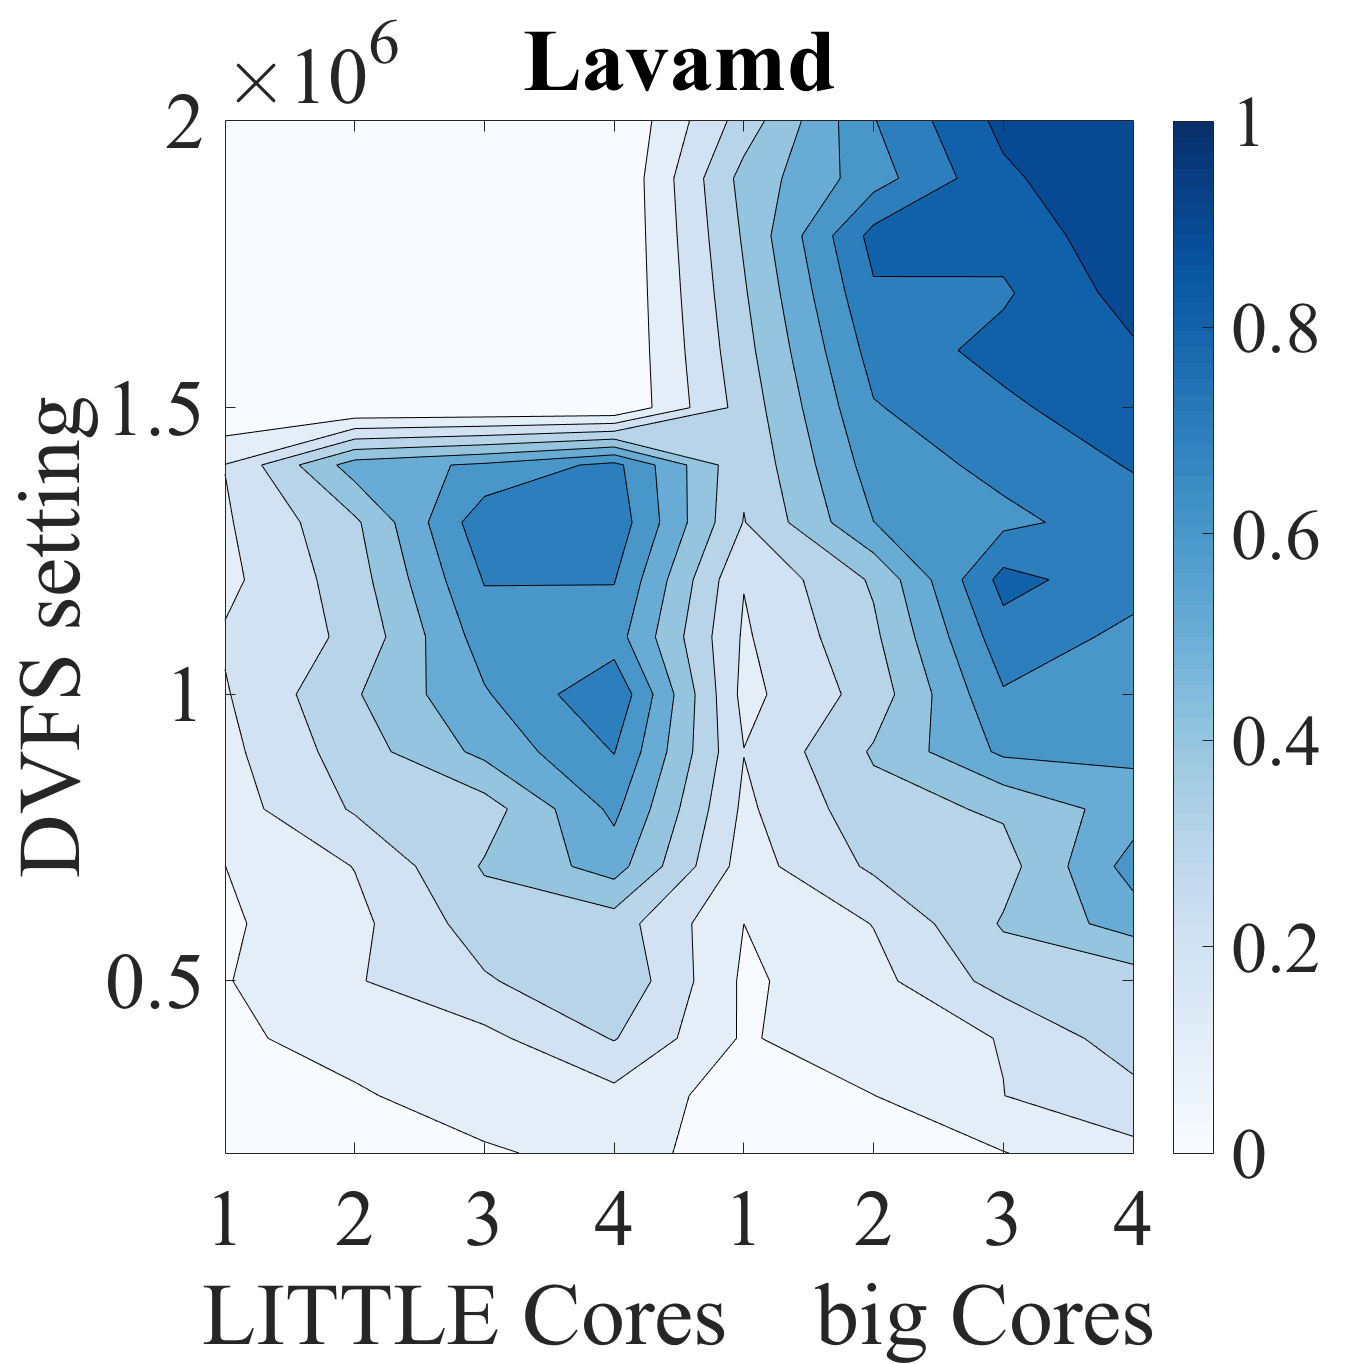
\includegraphics[width=.3\textwidth]{figures/lavamd.png}
    \label{fig:lavamd_contour}
  }
  \subfloat[]
  {
    \begin{tikzpicture}
\begin{centering}

\begin{groupplot}[
    group style={
        group name=plots,
        group size=1 by 1,
        xlabels at=edge bottom,
        xticklabels at=edge bottom,
        vertical sep=5pt
    },
height=4.1cm,
width=0.45\columnwidth,
xmajorgrids,
ymajorgrids,
grid style={dashed},
xmax=20,
yticklabel pos=left,
enlargelimits=false,
tick align = outside,
tick style={white},
xticklabel shift={-5pt},
yticklabel shift={-5pt},
ylabel shift={-2pt},
ylabel style={align=center},
unbounded coords=jump,
]

\nextgroupplot[ylabel={\scriptsize Performance (Normalized)}, % Performance
xlabel={\footnotesize Iteration},
ytick={0.0,0.5,1.0,1.5,2.0},
yticklabels={,0.25,0.5,1.0,1.5},
legend entries={,{\scriptsize $\mathsf{Generic~Model}$},{\scriptsize $\mathsf{LAVAMD model}$}},
legend style={fill=none,draw=none,at={(0.5,1.4)},anchor=north,legend columns=1,line width=3pt},
]

\addplot[thick, dashed, black] coordinates {(10,0) (10,1.5)};
\addplot[thick, solid, color=poet] table[x index=0,y index=1,col sep=tab] {img/image_text/lavamd-example.txt};
\addplot[thick, solid, color=cal] table[x index=0,y index=2,col sep=tab] {img/image_text/lavamd-example.txt};
\end{groupplot}
\end{centering}
\end{tikzpicture}
    \label{fig:lavamd_timeline}
  }
  \caption{(a) Contour plot for normalized performance for \texttt{Lavamd} algorithm for different configurations(b) Time-line for running \texttt{Lavamd}. \emph{Control} is running in isolation without an HBM based \emph{learning} mechanism which leads to oscillations in the performance.}
  \label{fig:learning-models}
\end{figure*}

\begin{figure}
  \subfloat[]
  {
    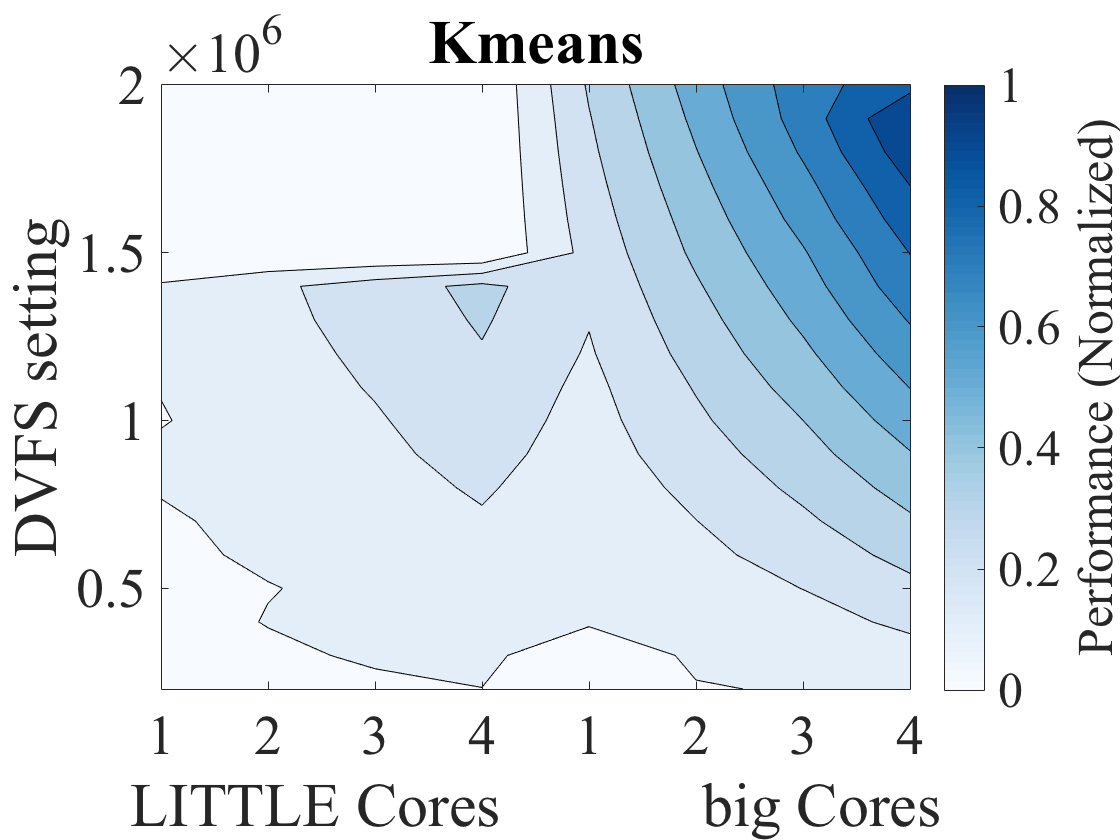
\includegraphics[width=.3\columnwidth]{figures/kmeans.png}
    \label{fig:kmeans_contour}
  }
  \subfloat[]
  {
    \begin{tikzpicture}
\begin{centering}

\definecolor{s1}{RGB}{228, 26, 28}
\definecolor{s2}{RGB}{55, 126, 184}
\definecolor{s3}{RGB}{77, 175, 74}
\definecolor{s4}{RGB}{152, 78, 163}
\definecolor{s5}{RGB}{255, 127, 0}

\begin{groupplot}[
    group style={
        group name=plots,
        group size=1 by 1,
        xlabels at=edge bottom,
        xticklabels at=edge bottom,
        vertical sep=5pt
    },
height=4cm,
width=1.3\columnwidth,
xmajorgrids,
ymajorgrids,
grid style={dashed},
xmin=0,
xmax=20,
yticklabel pos=left,
enlargelimits=false,
tick align = outside,
tick style={white},
xticklabel shift={-5pt},
yticklabel shift={-5pt},
ylabel shift={-2pt},
ylabel style={align=center},
unbounded coords=jump,
]

\nextgroupplot[ylabel={\footnotesize Performance \\ (Normalized)}, % Performance
%xtick={0,500,1000,1500,2000,2500,3000,3500,4000,4500},
ytick={0.0,0.5,1.0,1.5,2.0},
yticklabels={,0.5,1.0,1.5,2.0},
%xtick={0,30,60,120,160,200,240,280,320,480},
%xticklabels={,0,30,60,120,160,200,240,280,320,480},
%yticklabel style={font=\footnotesize},
xlabel={\footnotesize time (in sec)},
ymin=0,
ymax=1.5,
legend entries={,{$\mathsf{Learning}$},{$\mathsf{Control}$}},
legend style={draw=none,at={(0.5,1.3)},anchor=north,legend columns=4,
line width=5pt},
]

\addplot[thick, dashed, black] coordinates {(10,0) (10,1.5)};
\addplot[thick, solid, color=s4] table[x index=0,y index=1,col sep=tab] {img/image_text/kmeans-example.txt};
\addplot[thick, solid, color=s5] table[x index=0,y index=2,col sep=tab] {img/image_text/kmeans-example.txt};
%\addplot[thick, dashed, black] coordinates {(130,0) (130, 2)};
\end{groupplot}
\end{centering}

\end{tikzpicture}

    \label{fig:kmeans_timeline}    
  }
  \caption{(a) Contour plot for normalized performance for \texttt{Kmeans} algorithm for different configurations(b) Time-line for running \texttt{Kmeans} alone until 10 seconds, when another application. \emph{Learning} is running in isolation without an LCS based \emph{control} mechanism which leads to a performance drop which does not recover by itself.}
  \label{fig:learning-models}
\end{figure}
}
\begin{figure*}
  \subfloat[]
  {
    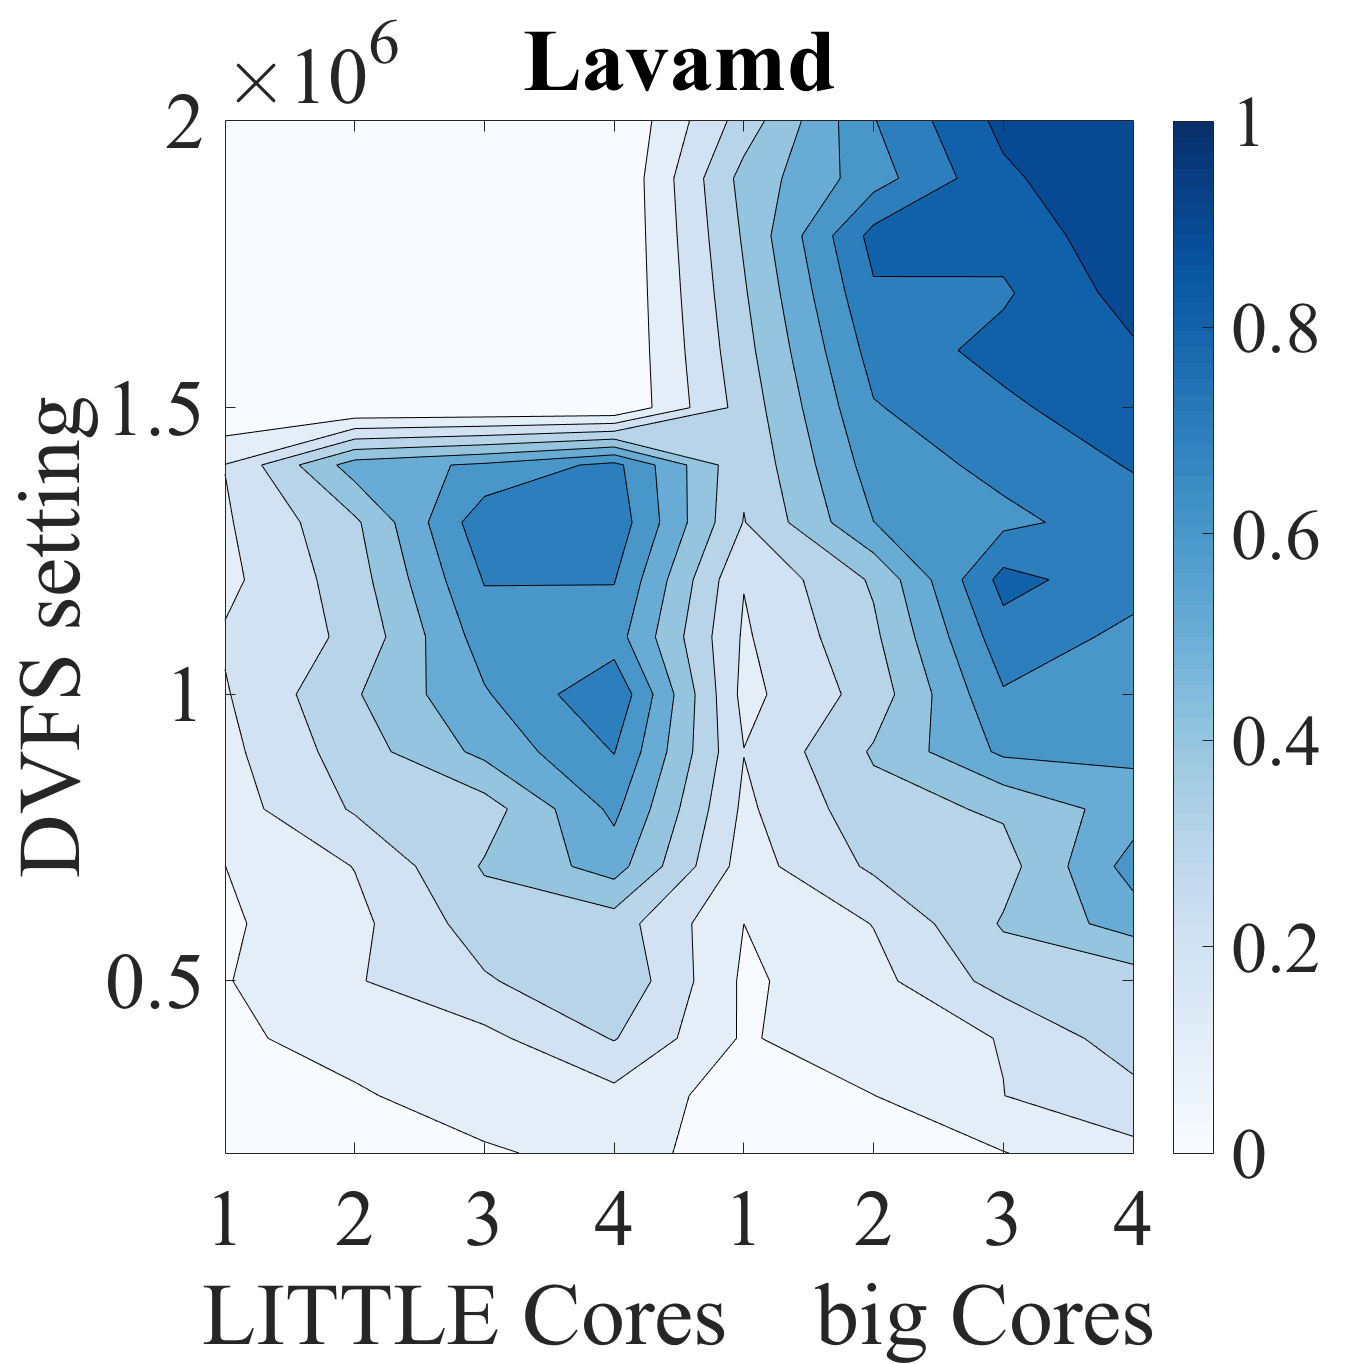
\includegraphics[width=.25\textwidth]{figures/lavamd.png}
    \label{fig:lavamd_contour}
  }
  \subfloat[]
  {
    \begin{tikzpicture}
\begin{centering}

\begin{groupplot}[
    group style={
        group name=plots,
        group size=1 by 1,
        xlabels at=edge bottom,
        xticklabels at=edge bottom,
        vertical sep=5pt
    },
height=4.1cm,
width=0.45\columnwidth,
xmajorgrids,
ymajorgrids,
grid style={dashed},
xmax=20,
yticklabel pos=left,
enlargelimits=false,
tick align = outside,
tick style={white},
xticklabel shift={-5pt},
yticklabel shift={-5pt},
ylabel shift={-2pt},
ylabel style={align=center},
unbounded coords=jump,
]

\nextgroupplot[ylabel={\scriptsize Performance (Normalized)}, % Performance
xlabel={\footnotesize Iteration},
ytick={0.0,0.5,1.0,1.5,2.0},
yticklabels={,0.25,0.5,1.0,1.5},
legend entries={,{\scriptsize $\mathsf{Generic~Model}$},{\scriptsize $\mathsf{LAVAMD model}$}},
legend style={fill=none,draw=none,at={(0.5,1.4)},anchor=north,legend columns=1,line width=3pt},
]

\addplot[thick, dashed, black] coordinates {(10,0) (10,1.5)};
\addplot[thick, solid, color=poet] table[x index=0,y index=1,col sep=tab] {img/image_text/lavamd-example.txt};
\addplot[thick, solid, color=cal] table[x index=0,y index=2,col sep=tab] {img/image_text/lavamd-example.txt};
\end{groupplot}
\end{centering}
\end{tikzpicture}
    \label{fig:lavamd_timeline}
  }
  \subfloat[]
  {
    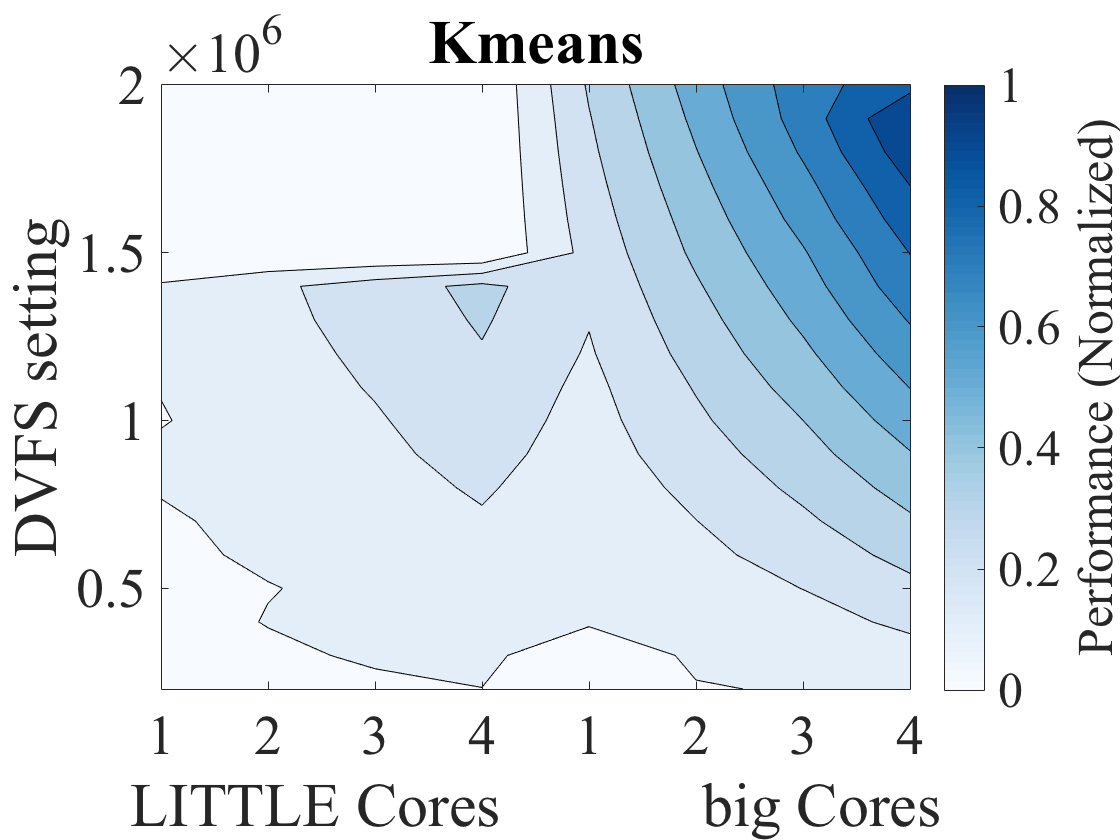
\includegraphics[width=.25\textwidth]{figures/kmeans.png}
    \label{fig:kmeans_contour}
  }
  \subfloat[]
  {
    \begin{tikzpicture}
\begin{centering}

\definecolor{s1}{RGB}{228, 26, 28}
\definecolor{s2}{RGB}{55, 126, 184}
\definecolor{s3}{RGB}{77, 175, 74}
\definecolor{s4}{RGB}{152, 78, 163}
\definecolor{s5}{RGB}{255, 127, 0}

\begin{groupplot}[
    group style={
        group name=plots,
        group size=1 by 1,
        xlabels at=edge bottom,
        xticklabels at=edge bottom,
        vertical sep=5pt
    },
height=4cm,
width=1.3\columnwidth,
xmajorgrids,
ymajorgrids,
grid style={dashed},
xmin=0,
xmax=20,
yticklabel pos=left,
enlargelimits=false,
tick align = outside,
tick style={white},
xticklabel shift={-5pt},
yticklabel shift={-5pt},
ylabel shift={-2pt},
ylabel style={align=center},
unbounded coords=jump,
]

\nextgroupplot[ylabel={\footnotesize Performance \\ (Normalized)}, % Performance
%xtick={0,500,1000,1500,2000,2500,3000,3500,4000,4500},
ytick={0.0,0.5,1.0,1.5,2.0},
yticklabels={,0.5,1.0,1.5,2.0},
%xtick={0,30,60,120,160,200,240,280,320,480},
%xticklabels={,0,30,60,120,160,200,240,280,320,480},
%yticklabel style={font=\footnotesize},
xlabel={\footnotesize time (in sec)},
ymin=0,
ymax=1.5,
legend entries={,{$\mathsf{Learning}$},{$\mathsf{Control}$}},
legend style={draw=none,at={(0.5,1.3)},anchor=north,legend columns=4,
line width=5pt},
]

\addplot[thick, dashed, black] coordinates {(10,0) (10,1.5)};
\addplot[thick, solid, color=s4] table[x index=0,y index=1,col sep=tab] {img/image_text/kmeans-example.txt};
\addplot[thick, solid, color=s5] table[x index=0,y index=2,col sep=tab] {img/image_text/kmeans-example.txt};
%\addplot[thick, dashed, black] coordinates {(130,0) (130, 2)};
\end{groupplot}
\end{centering}

\end{tikzpicture}

    \label{fig:kmeans_timeline}    
  }
  \caption{(a) Performance for \texttt{lavamd} as a function of
    configuration. (b) Managing \texttt{lavamd}'s performance:
    \emph{Learning} navigates the complicated configuration space, but
    \emph{control}'s simple model leads to oscillation. (c)
    Performance for \texttt{kmeans} as a function of configuration.
    (d) Managing \texttt{kmeans}' performance when another application
    starts: \emph{Control} detects the change and adapts, but
    \emph{learning} has no mechanism to handle these dynamics.}
  \label{fig:learning-models}
\end{figure*}



We present two simple examples to illustrate the complementary
strengths and weaknesses of learning and control.  We use mobile
development boards featuring Samsung's Exynos 5 Octa with an ARM
big.LITTLE architecture that has four energy-efficient LITTLE cores
and four high-performance big cores.  Each cluster can be set to
different frequencies, leading to a large configuration space for
assigning resources to multi-threaded applications.

\PUNT{Each configuration (assignment of cores and frequencies) has
  different performance for different applications.}
\figsref{fig:lavamd_contour}{fig:kmeans_contour} show how performance
varies as a function of both resource usage and application.  The
figures show cores on the x-axis and frequency on the y-axis, with
darker colors representing higher performance.  The presence of local
minima and maxima mean that the function from resource usage to
performance is non-convex.  Therefore, simple gradient ascent/descent
methods are not suitable to navigating these configuration spaces.
Additionally, \texttt{lavamd} has a significantly more complicated
configuration space than \texttt{kmeans}.

\PUNT{
\begin{figure}
\centering
%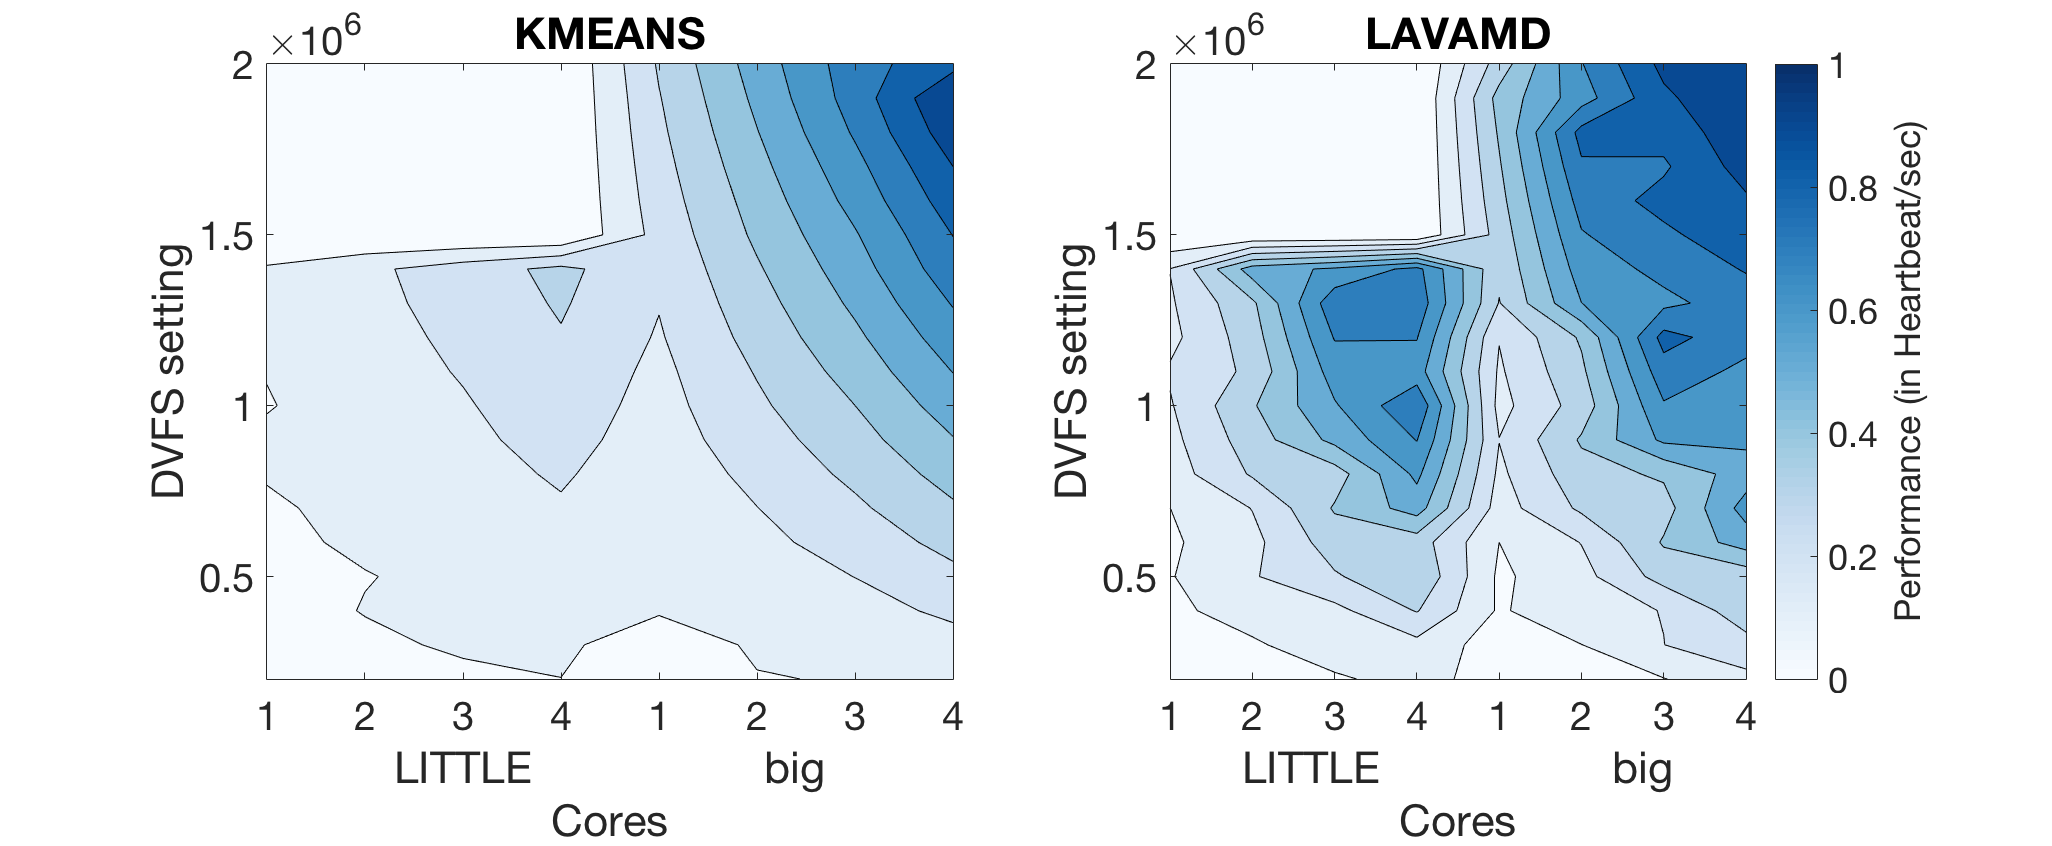
\includegraphics[width=\paperwidth,scale=0.5]{figures/performance-contour2.png}
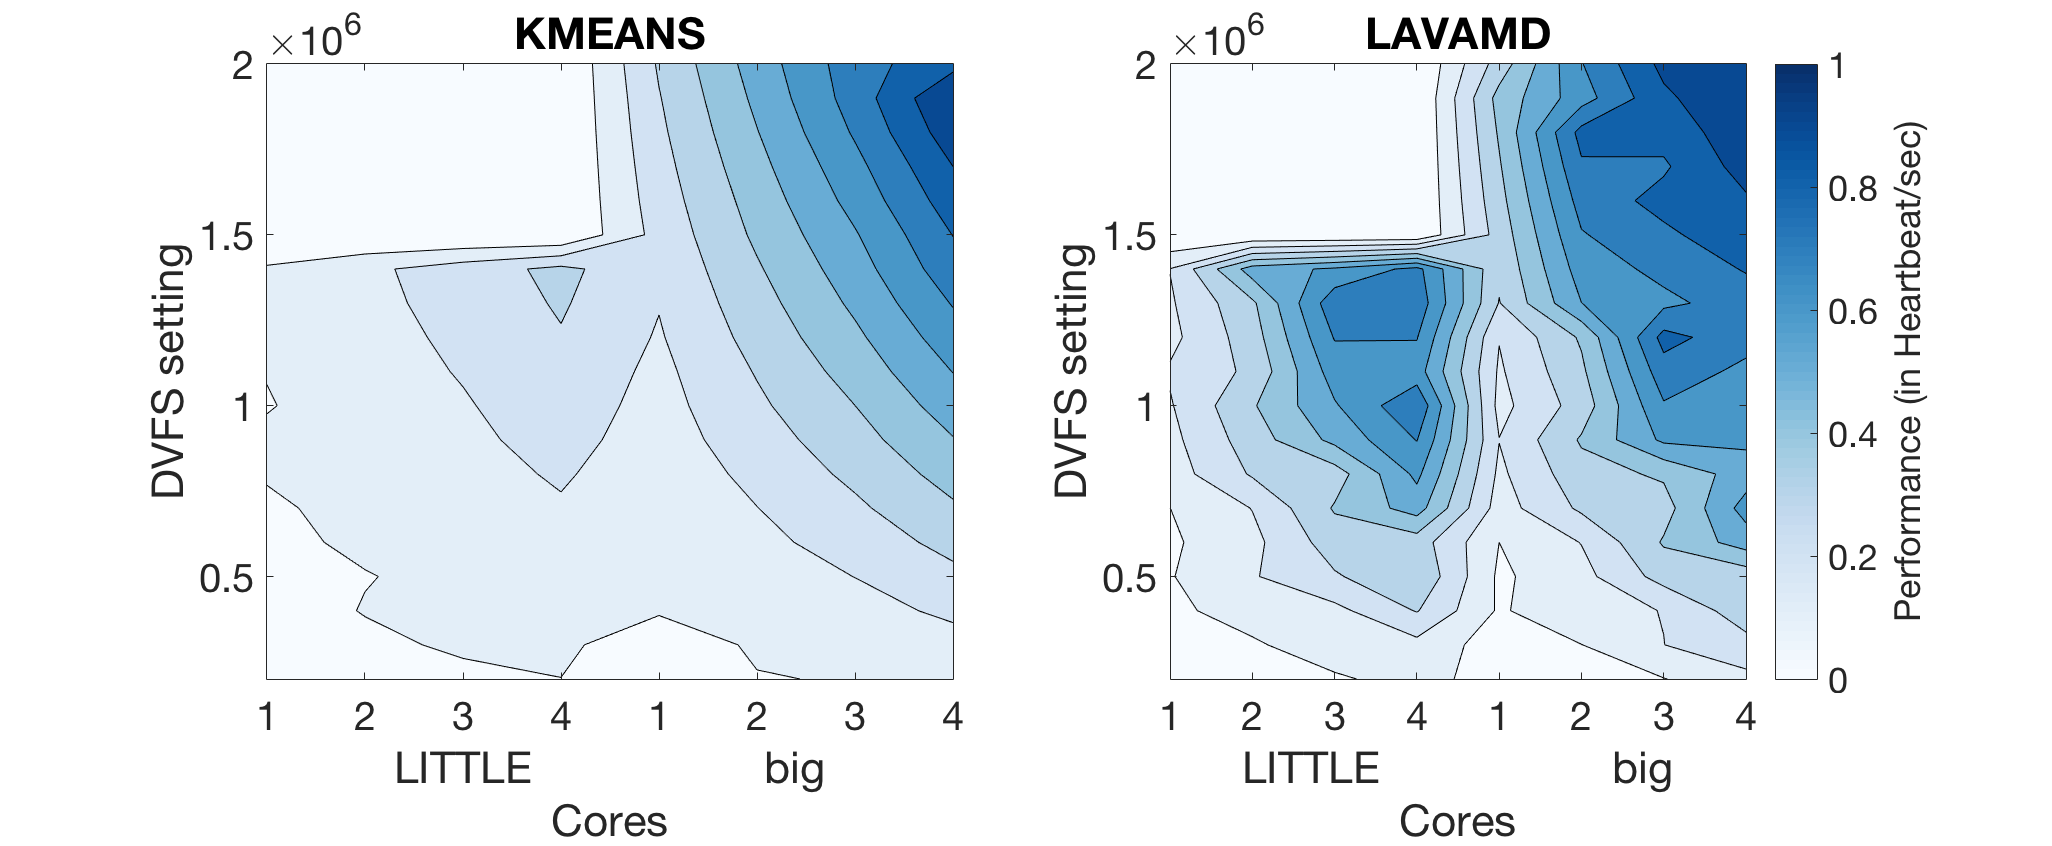
\includegraphics[width=\columnwidth]{figures/performance-contour2.png}
%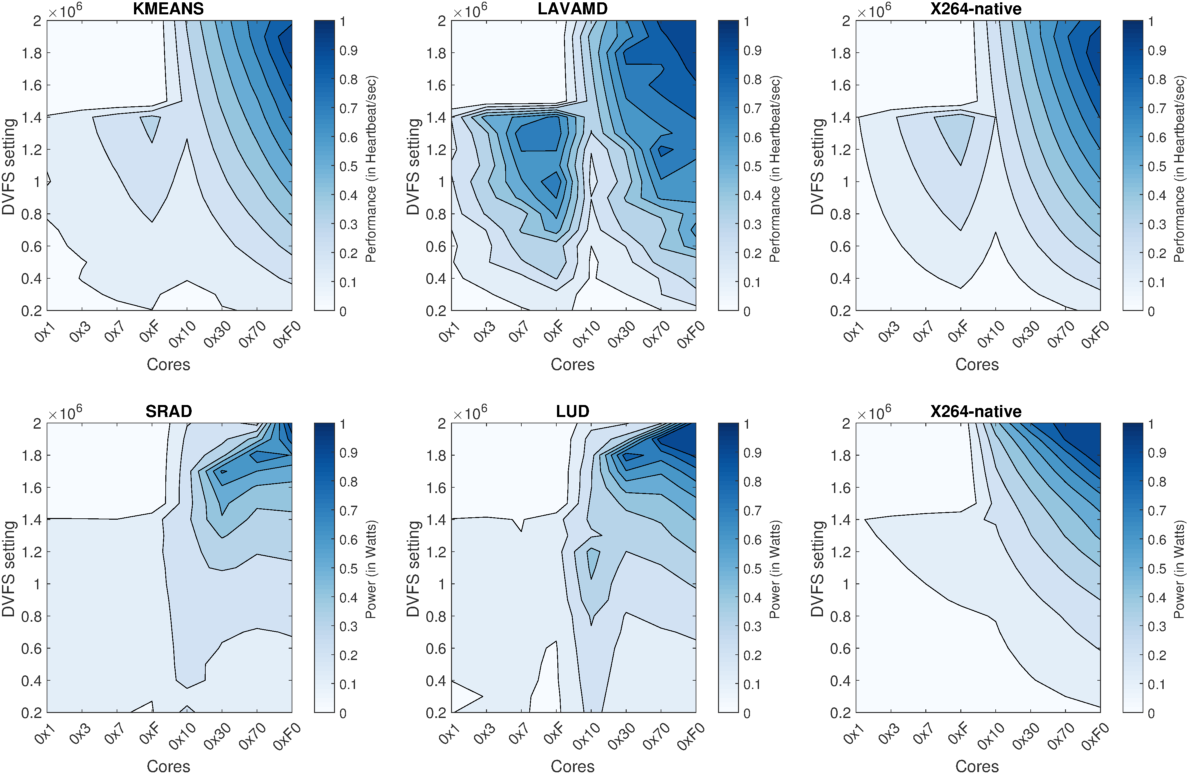
\includegraphics[scale=0.4]{figures/sample-contour3.png}
\caption{Contour plots showing performance as a function of core
  number, type, and speed.}
  \label{fig:contour}
\end{figure}
}

We consider prior \emph{learning} and \emph{control} approaches.  LEO,
a hierarchical Bayesian learner, estimates application performance as
a function of its resource usage \cite{LEO}. POET, a control system,
adjusts resource usage to meet application performance requirements
with minimal energy \cite{POET}.  This section develops intuition
about when one approach performs better than the other, motivating our
proposal to combine the two.

\subsection{\emph{Learning} Complexity}
Many machine learning approaches have been proposed to estimate
application performance in a variety of scenarios
\cite{reddiHPCA2013,LeeBrooks2006,CPR,ParallelismDial,Flicker,LeeBrooks,Koala}.
Machine learning is well suited to building models of complicated
systems like those shown in
\figsref{fig:lavamd_contour}{fig:kmeans_contour}.

To demonstrate how well learning manages complexity, we consider
meeting a performance requirement for \texttt{lavamd}, which has a
complicated configuration space.  We launch the application and use
either \emph{learning} or \emph{control} to meet a performance
requirement with minimal energy.  The \emph{learning} approach
estimates all configurations' performance and power and then uses the
lowest power configuration that delivers the required performance.
The \emph{control} approach has a generic model of power/performance
frontiers (similar to \texttt{kmeans}) and it constantly measures
performance and adjusts resource usage according to this generic
model.  \PUNT{While many controllers use linear models, POET uses a
  convex model and handles some non-linearities; however, it is
  sensitive to local maxima.}

\figref{fig:lavamd_timeline} shows the results of controlling 30
iterations of \texttt{lavamd} to meet the performance requirement.
The x-axis shows iteration number and the y-axis shows normalized
performance.  The learning approach achieves the goal, but the
controller oscillates wildly around it, sometimes not achieving the
goal and sometimes delivering performance that is too high (and wastes
energy). The oscillations occur because the controller adjusts
resources based on an incorrect (over-simplified) model of the
configuration space. Hence, the \emph{learner}'s ability to handle
complex models is crucial for reliable performance in this example.

%This result may be somewhat counter-intuitive.  The problem is that the controller cannot handle the complexity of \texttt{lavamd}.  One way to fix this problem would be to build a custom controller just for this application, but that controller would not be useful for other applications.  In contrast, the learner can find the local maxima in the configuration space, and as this application has no phase changes or other dynamics, the one configuration that the learner finds is suitable for the entire application.

\subsection{\emph{Controlling} Dynamics}
We now consider a dynamic environment.  We begin with \texttt{kmeans}
as the only application running on the system.  Halfway through its
execution, we launch a second app on a big core, dynamically altering
resource availability.

\figref{fig:kmeans_timeline} shows the results of this experiment.
The vertical dashed line represents when the second application
begins.  The figure clearly shows the benefits of a control system in
this dynamic scenario.  After a small dip in performance, the
controller returns it back to the desired level.  The learning system
however, does not have any inherent mechanism to measure the change or
adapt to the altered performance.  While we could theoretically
relearn the configuration space whenever the environment changes,
doing so is impractical.

Control systems are a light-weight mechanisms for managing such
dynamics \cite{Hellerstein2004a}. Control systems are resilient to
scale change in the system performance or power.  Many dynamic changes
reduce all configurations' performance almost uniformly, changing the
magnitude of performance without altering the relative difference
between configurations.  For this reason, control systems have proven
especially useful in webservers with fluctuating request rates
\cite{Horvarth,LuEtAl-2006a,SunDaiPan-2008a} and multimedia
applications with dynamically varying inputs
\cite{TCST,Agilos,grace2}.

%%
\PUNT{
\begin{figure}
\centering
%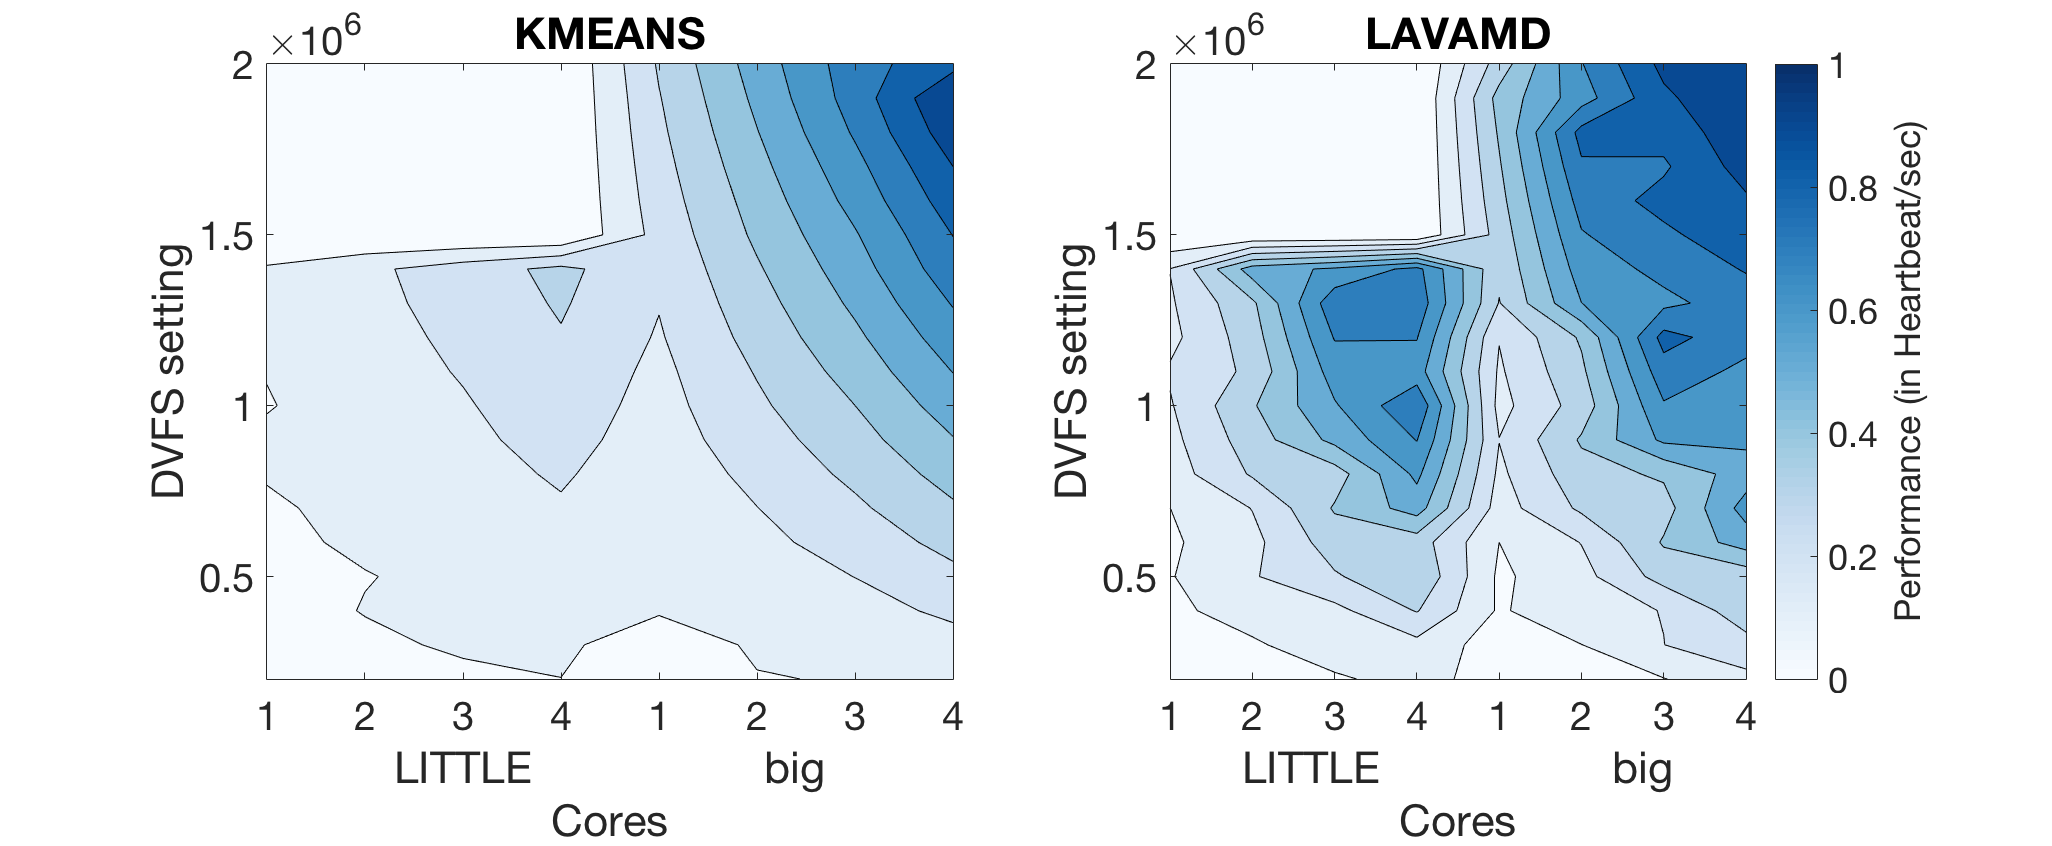
\includegraphics[width=\paperwidth,scale=0.5]{figures/performance-contour2.png}
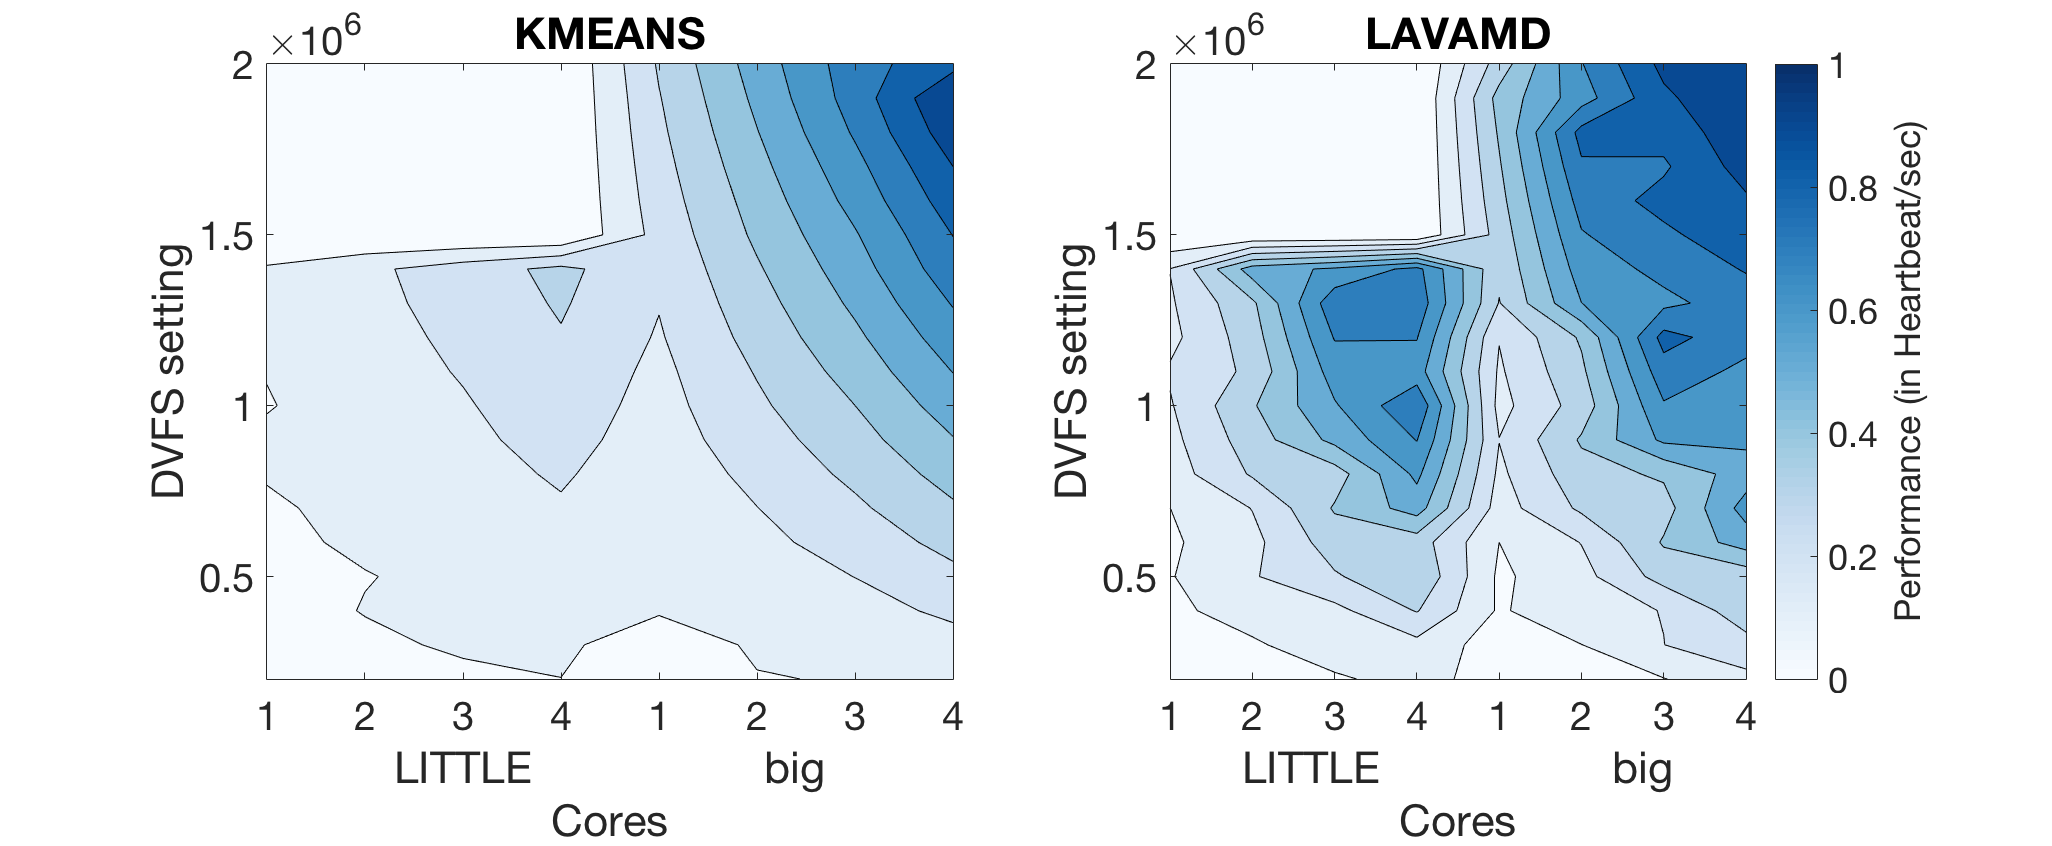
\includegraphics[width=\columnwidth]{figures/performance-contour2.png}
%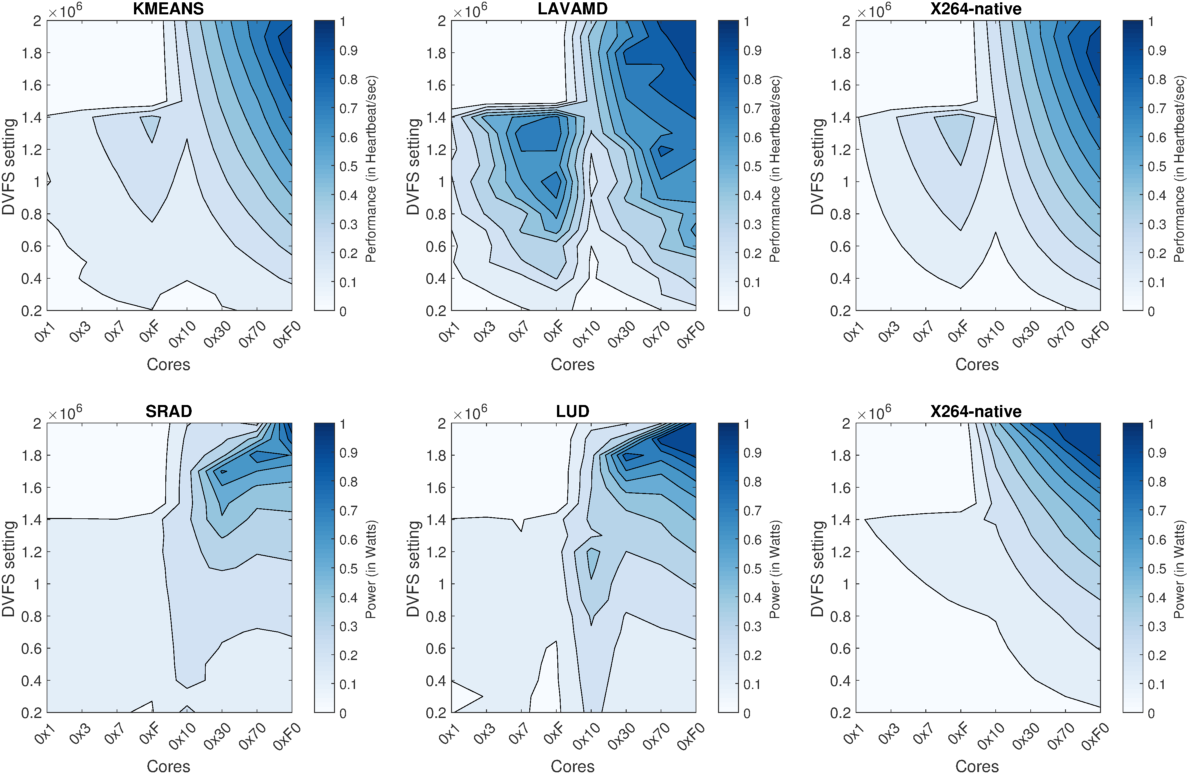
\includegraphics[scale=0.4]{figures/sample-contour3.png}
\caption{Contour plots showing performance as a function of core
  number, type, and speed.}
  \label{fig:contour}
\end{figure}

\begin{figure}[t]
  \begin{tikzpicture}
\begin{centering}

\definecolor{s1}{RGB}{228, 26, 28}
\definecolor{s2}{RGB}{55, 126, 184}
\definecolor{s3}{RGB}{77, 175, 74}
\definecolor{s4}{RGB}{152, 78, 163}
\definecolor{s5}{RGB}{255, 127, 0}

\begin{groupplot}[
    group style={
        group name=plots,
        group size=1 by 1,
        xlabels at=edge bottom,
        xticklabels at=edge bottom,
        vertical sep=5pt
    },
height=3.5cm,
width=0.95\columnwidth,
xmajorgrids,
ymajorgrids,
grid style={dashed},
xmin=0,
xmax=20,
yticklabel pos=left,
enlargelimits=false,
tick align = outside,
tick style={white},
xticklabel shift={-5pt},
yticklabel shift={-5pt},
ylabel shift={-2pt},
ylabel style={align=center},
unbounded coords=jump,
]

\nextgroupplot[ylabel={\footnotesize Performance \\ (Normalized)}, % Performance
%xtick={0,500,1000,1500,2000,2500,3000,3500,4000,4500},
ytick={0.0,0.5,1.0,1.5,2.0},
yticklabels={,0.5,1.0,1.5,2.0},
%xtick={0,30,60,120,160,200,240,280,320,480},
%xticklabels={,0,30,60,120,160,200,240,280,320,480},
yticklabel style={font=\footnotesize},
ymin=0,
ymax=1.5,
legend entries={,{$\mathsf{Learning}$},{$\mathsf{Control}$}},
legend style={draw=none,at={(0.5,1.4)},anchor=north,legend columns=4,line width=5pt},
]

\addplot[thick, dashed, black] coordinates {(10,0) (10,1.5)};
\addplot[thick, solid, color=s4] table[x index=0,y index=1,col sep=tab] {img/image_text/kmeans-example.txt};
\addplot[thick, solid, color=s5] table[x index=0,y index=2,col sep=tab] {img/image_text/kmeans-example.txt};
%\addplot[thick, dashed, black] coordinates {(130,0) (130, 2)};
\end{groupplot}
\end{centering}

\end{tikzpicture}

   \vskip -1em
  \caption{Performance Control for KMEANS}
  \label{fig:kmeans-example}
\end{figure}
}





\section{\SYSTEM{}: Learning Control}
\label{sec:framework}


\PUNT{To do so, we must quickly build a model of the new application
  and then control its resource usage such that it meets a desired
  performance target with minimal energy.}

\begin{figure}
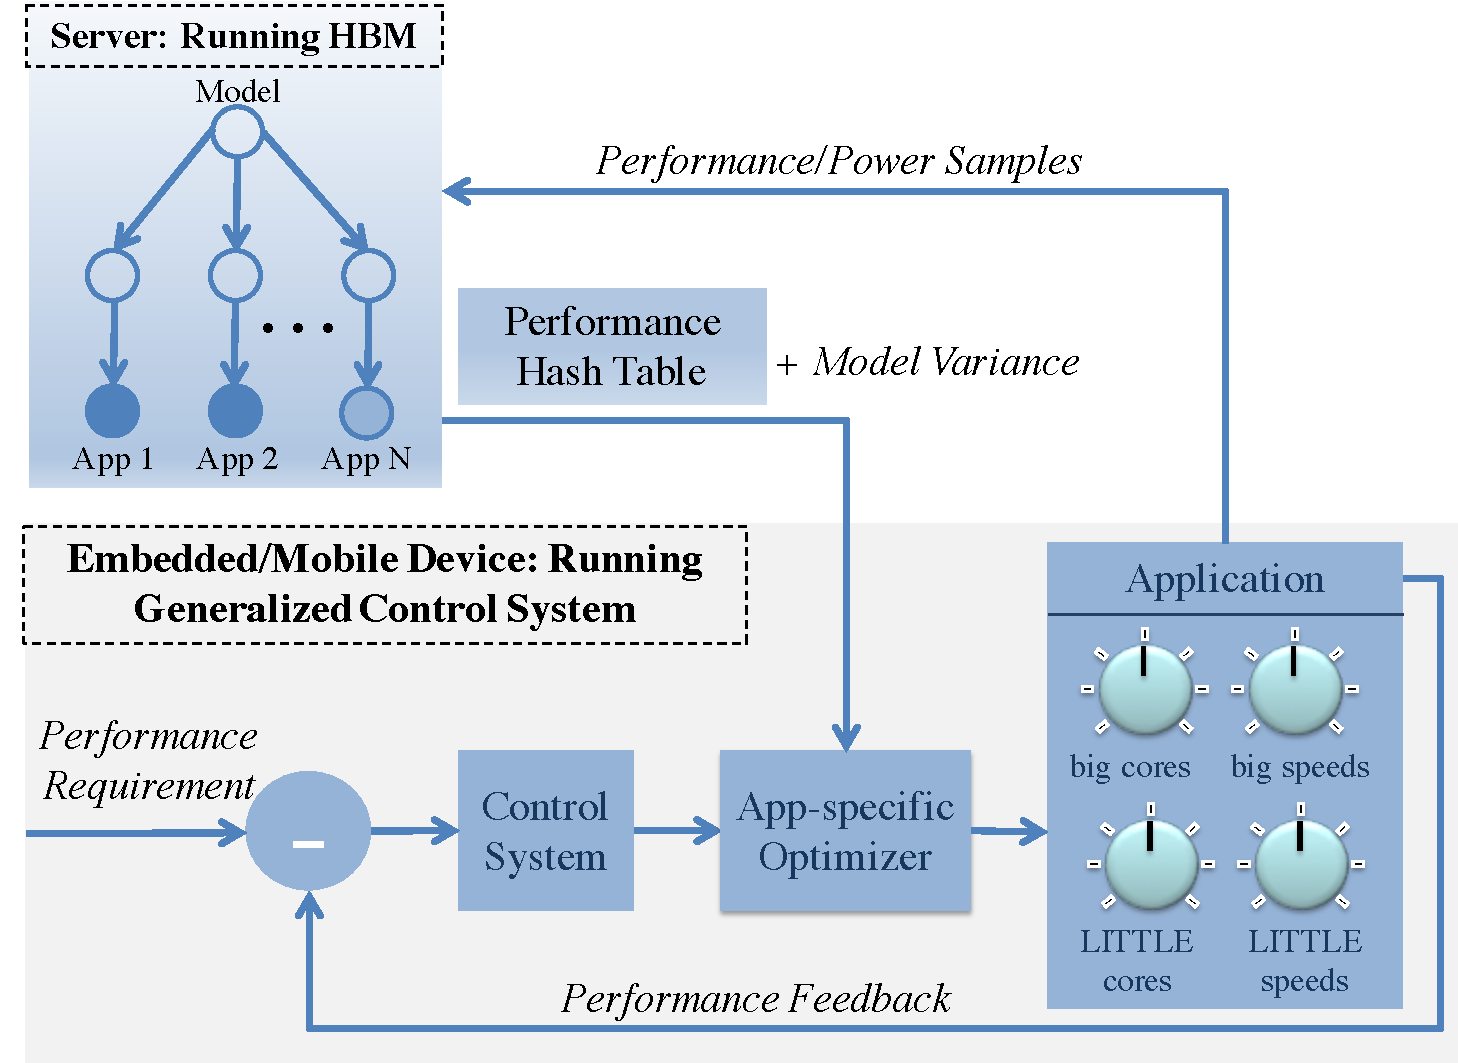
\includegraphics[width=\columnwidth]{figures/ControlLearning2.pdf}
\caption{Overview of \SYSTEM{}.}
\label{fig:overview}
\end{figure}


Our goal is control theoretic resource management for streaming
applications running on embedded or mobile devices, but assuming no
assume no prior knowledge of the application.  \figref{fig:overview}
shows \SYSTEM{}'s approach to this problem.  On the local device, a
generalized control system (GCS) allocates resources to the new
application to meet its specified performance goal with minimal
energy.  The GCS starts with a generic resource model, allocates
resources according to that model, and records performance and power
for a small number of configurations.  The recorded values are sent to
a remote server which runs a hierarchical Bayesian model (HBM).  The
HBM estimates the application's performance and power in all other
configurations and extracts those that are Pareto-optimal in the
performance/ power tradeoff space.  These configurations are packaged
in a special data structure -- the performance hash table (PHT) -- and
sent to the GCS.  Using the PHT, the GCS selects an energy minimal
resource configuration in constant time ($O(1)$).  The server also
sends back the model's variance, which the GCS uses to customize
control to the model's uncertainty. By communicating variance,
\SYSTEM{} guarantees convergence to the performance goal even though
it starts with no prior knowledge of the streaming application.

\PUNT{
The remainder of this section details \SYSTEM{}.  We begin by
describing a typical control design for a computer system and
illustrate how it fails to generalize.  We then describe \SYSTEM{}'s
generalized control system.  Next we discuss how \SYSTEM{} turns the
generalized control signal into specific resource configurations using
a model.  We then describe how to use a hierarchical Bayesian model to
estimate resource performance and power tradeoffs.  We then describe
the performance hash table that encodes the learned model. We conclude
with some brief analysis of the approach, with detailed analysis
provided in an appendix.
}

\subsection{Traditional Control for Computing}
\PUNT{
A controller has a performance goal (corresponding to a
quality-of-service or real-time constraint) and adjusts system resource
usage to see that the goal is met. Following is the general formulation for a controller, where the response is assumed to be linearly related to the effect.
\begin{equation}
  effect(t) = \alpha \cdot response(t-1) + \delta \label{eqn:clock}
\end{equation}
A control system might adjust processor frequency to ensure that a performance
goal is met \cite{lefurgy2008power}.  Even better, an optimal controller would
use the minimal clockspeed to meet the performance requirement.


To turn clockspeed into performance a controller needs a model
relating these two values.  A physical model, directly mapping clockspeed to performance
is difficult -- a hypothetical model might account for instruction
mixes, memory hierarchy, memory latency, synchronization overheads,
etc.  Building such a model is tedious and error-prone process and
that is before we address system dynamics (\eg applications
transitioning from memory to compute bound).  Instead, control systems
use relatively simple difference models\footnote{Continuous time
  systems would use differential equations, but as time in computers
  is inherently discretized we restrict ourselves to discussion of
  difference equations which are appropriate for discrete time
  systems.}.
}

%example difference model -- built into the controller

\PUNT{

Continuing the example of controlling performance with clockspeed, a
simple model appropriate for control would be to assume that the
performance is a linear function of the clockspeed:
\begin{equation}
  perf(t) = \alpha \cdot clockspeed(t-1) + \delta \label{eqn:clock}
\end{equation}
Here, the observed performance $perf(t)$ is predicted as some constant
$\alpha$ times the clockspeed applied at the previous time step,
$clockspeed(t-1)$, plus some noise, $\delta$ drawn from a Gaussian
distribution.  This simple linear difference model ignores low-level
details like instruction mix, and instead uses feedback, predicting
behavior of the next time step as a function of the previous time
step.  Using the relationship of \eqnref{clock}, we can synthesize a
simple controller that is provably convergent to the desired
performance:
\begin{eqnarray}
  error(t) &=& goal - perf(t) \label{eqn:clock-error} \\
  clockspeed(t) &=& clockspeed(t-1) - \frac{error(t)}{\alpha}
  \label{eqn:clock-control}
\end{eqnarray}
}


Using traditional control design, we can turn LAVAMD's model -- from
\figref{fig:lavamd_model} -- into a controller.  The model follows
directly from the linear fit:
\begin{equation}
  perf(t) = 2.95 \times 10^{-6} \cdot clock(t-1) + \delta \label{eqn:clock}
\end{equation}
This model states the observed $perf(t)$ is the slope of our model
times the clockspeed applied at the previous time step, $clock(t-1)$,
plus some Gaussian noise $\delta$.  This simple linear difference
model ignores low-level details like instruction mix, and instead uses
feedback, predicting behavior of the next time step as a function of
the previous time step.  Using \eqnref{clock}, we synthesize a simple
controller that is provably convergent to the $goal$ performance
\cite{ICSE2014}:
\begin{eqnarray}
  error(t) &=& goal - perf(t) \label{eqn:clock-error} \\
  clock(t) &=& clock(t-1) - \frac{error(t)}{ 2.95 \times 10^{-6}}
  \label{eqn:clock-control}
\end{eqnarray}



% Can we make the model a tunable parameter?
The controller design in \eqnref{clock-control} provides formal
guarantees that it will converge to the desired performance ($goal$ in
\eqnref{clock-error}) and it bounds convergence time.  These
guarantees, however, are predicated on the model's accuracy; \ie how
well the slope in \figref{fig:lavamd_model} approximates measured
performance.  This value is highly dependent on the particular
application under control.  This model will not work for applications
that are memory-bound and do not speed up with increasing clockspeed.
As we add more resources to the controller we turn the scalara
equations of this example into matrix equations
\cite{METE,josep-isca2016}.  Whether scalar or matrix, the equations
and the formal guarantees they embody are reliant on accurate models
of resource interaction.  Since we cannot build one model for all
applications, we want to tune the control models to individual
applications.

\subsection{Generalized Control System}
In the above example, the controller is application-specific because
it directly incorporates the slope of the model into the control
equations.  Our goal is to build a controller where those key
parameters can be tuned online.  To do so, we use the classic computer
science trick of adding a layer of indirection as illustrated in
\figref{fig:overview}.  Instead of directly controlling resources
using an application-dependent model, we will control \emph{speedup}
and pass that speedup value to a separate module that turns desired
speedup into an energy-minimal resource configuration using the
learned models.  We first describe our formulation for controlling
speedup and then converting that speedup into resource allocations.

\subsubsection{Controlling Speedup}
Analogous to \eqnref{clock} we write a simple difference model
relating speedup to performance:
\begin{equation}
  perf(t) = b \cdot speedup(t-1) + \delta \label{eqn:speedup}
\end{equation}
where $b$ is the application's \emph{base speed}: defined as the speed
when all resources are available.  While $b$ is application specific,
it is easy to measure online, by simply allocating all resources. Such
a configuration should not violate any performance constraints
(although it is unlikely to be energy efficient) so it is safe to take
this measurement without risk of violating performance constraints.

With this model, the control law is simply:
\begin{eqnarray}
  error(t) &=& goal - perf(t) \label{eqn:speedup-error} \\
  speedup(t) &=& speedup(t-1) - \frac{error(t)}{b}
  \label{eqn:speedup-control}
\end{eqnarray}
which states that the speedup at time $t$ is a function of the
previous speedup, the error at time $t$ and the base speed.  This is a
very simple \emph{deadbeat} controller that provides all the standard
control theoretic formal guarantees.


By measuring base speed online while the application runs, we tune the
control to a specific application; using this definition of base
speed, most speedups will be less than one.  We can further generalize
\eqref{eqn:speedup-control} as:
\begin{equation}
speedup(t) = speedup(t-1) - \frac{1 - p}{b}.error(t)
\end{equation}
where $0 \le p < 1$ is a pole of the controller's characteristic
equation.  At small values of $p$ the controller will work to
eliminate error very quickly, but it may overreact to noise or
inaccuracies in the model.  Larger values of $p$ make the system more
robust at the cost of reduced convergence time.  \emph{Dynamically
  setting the pole to the HBM's output will be a key of combining
  control and learning.} First, however, we address the challenging
problem of converting an abstract speedup into an actual resource
allocation.


\subsubsection{Converting Speedup to Resource Allocation}
We need to map \eqnref{speedup-control}'s speedup into a resource
allocation.  On our example ARM big.LITTLE architecture that
specifically means mapping speedup into an allocation of big and small
as well as a speed for both (on our system clocks big and little cores
separately).

The primary challenge is that the HBM produces a discrete non-linear
function of resource usage into speedup and powerup, while
\eqnref{speedup-control} is a continuous linear function.  We bridge
this divide by assigning time to resource allocations such that the
average speedup over a control interval is that produced by
\eqnref{speedup-control}.

We call an assignment of time to resources a schedule. There are
typically many schedules that meet a particular performance
requirement and we want to find a minimal energy schedule. Given a
time interval $T$, a speedup requirement $speedup(t)$ to average over
the time interval, and a configuration set of size $C$ , we formalize
this problem as:
\begin{eqnarray}
  \minimize_{\mathbf{\tau} \in \R^{C}} && \sum_{c=0}^{C-1} \tau_c \cdot p_c \label{eqn:power}  \\
  \st %&& \nonumber\\
  && \sum_{c=0}^{C-1} \tau_c \cdot s_c =  speedup(t)T \label{eqn:work} \\
  && \sum_{c=0}^{C-1} \tau_c =  T \label{eqn:deadline} \\
  && 0 \le \tau_c \le T, \qquad \forall c \in \{0,\ldots,C-1\} \label{eqn:time}
\end{eqnarray}
where $p_c$ and $s_c$ are configuration $c$'s estimated powerup and
speedup; $\tau_c$ is the time to spend in configuration $c$.
\eqnref{power} simply states that the objective is to minimize energy
(power times time).  \eqnref{work} states that the average speedup
must be maintained, while \eqnref{deadline} requires the time to be
fully utilized.  \eqnref{time} simply avoids negative time.


\subsection[Learning Power/Performance Tradeoffs]{Hierarchical Bayesian Models}
\PUNT{
\begin{figure}
\centering
  \subfloat[]
  {
    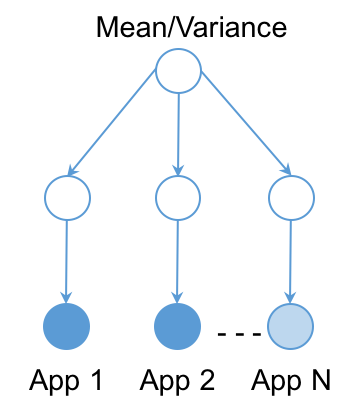
\includegraphics[width=.2\textwidth]{figures/HBM.png}
  }
  \caption{ A Hierarchical Bayesian model.  The arrows represent
    dependences, circles are random variables, white circles are
    hidden variables that cannot be observed and must be learned,
    solid circles represent fully observed data, and shaded circles
    represent partially observed data.}
\label{fig:learning-models}
\end{figure}

\begin{figure*}

  \subfloat[]
  {
    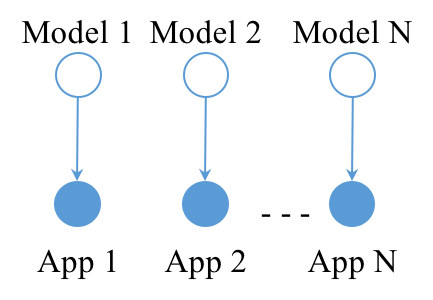
\includegraphics[width=.33\textwidth]{figures/Online.png}
    \label{fig:online}
  }
  \subfloat[]
  {
    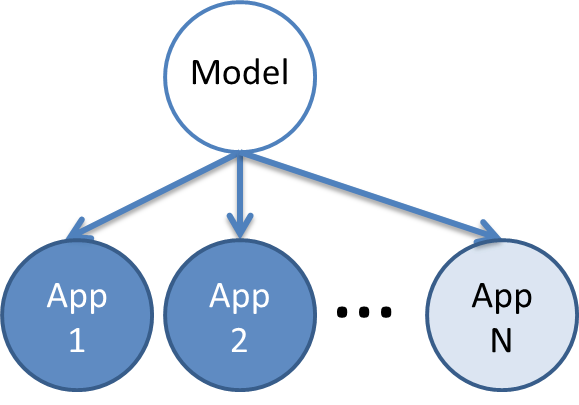
\includegraphics[width=.33\textwidth]{figures/Offline.png}
    \label{fig:offline}
  }
  \subfloat[]
  {
    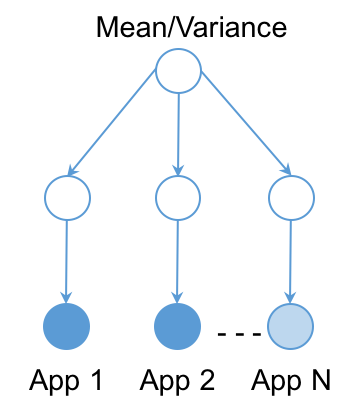
\includegraphics[width=.33\textwidth]{figures/HBM.png}
    \label{fig:HBM}
  }
  \caption{ Comparison of online (a) offline (b) and hierarchical
    Bayesian models (c).  The arrows represent dependences, circles
    are random variables, white circles are hidden variables that
    cannot be observed and must be learned, solid circles represent
    fully observed data, and shaded circles represent partially
    observed data.  The online model is concerned only with the
    current application (labeled N), the offline model combines all
    observations into one model, and the HBM builds per-application
    models, but makes them conditionally dependent on one another so
    that prior observations can be used to increase the accuracy of
    the model built for application N.}
\label{fig:learning-models}
\end{figure*}
}

Assuming no prior knowledge of the application, we estimate its power
($p_c$) and performance ($r_c$) in configuration $c$.
\PUNT{Specifically, we take observations of performance and power in a
  resource configuration and predict (1) how future applications will
  perform or (2) how different resource allocations affect the current
  application.}  \SYSTEM{} uses a hierarchical Bayesian model (HBM) to
turn observations of an application's performance and power into
predictions about how other, unobserved resource allocations will
affect performance and power.  The HBM provides a statistically sound
framework for learning across applications and devices; \ie{} it
handles the non-convex tradeoff spaces heterogeneity produces (\eg{}
\figref{fig:lavamd_contour}).

The HBM provides balance between completely online approaches -- which
consider only the current application -- and offline approaches --
which consider only prior applications approaches.  \PUNT{ Each
  application has its own model, allowing specificity, but these
  models are conditionally dependent on some underlying probability
  distribution with a hidden mean and co-variance matrix.  In
  practice, the HBM will estimate a model for a new application using
  a small number of observations and combining those observations with
  the large number of observations previously made of similar
  applications.  Rather than over-generalizing, the HBM will use only
  similar applications to learn models.  In addition, the HBM's
  accuracy increases as more applications are observed because more
  different types of behavior are represented in the pool of prior
  knowledge.  Of course, the computational complexity of learning also
  increases with increasing applications, but this is why we offload
  the learning to a remote server.  } Consider a simplified example.
Suppose we have observed many prior applications, all of which are
either completely compute-bound or completely memory-bound, and we
have an equal number of both.  The only resource we can allocate is
clockspeed, which will increase the performance of compute-bound
applications, but not memory-bound ones.  When we need to work with a
new application, we need to estimate its response to clockspeed.  The
online model does not use prior knowledge, but will observe many
different clock speeds for the new application, leading to high
overhead.  A fully offline model predicts the mean response of prior
applications, meaning it will over-allocate speed to memory-bound
applications and under-allocate to compute-bound ones.  The HBM takes
a small number of observations and combines those with prior
knowledge: if the new observations show that clockspeed has no effect
on performance the HBM will use only the prior memory bound
applications to build its model, otherwise, it will use the
compute-bound applications.  In practice, the HBM can learn much more
complicated tradeoffs by combining observations of the new application
with prior knowledge of different types of behavior.

\PUNT{
When selecting a learning framework we must find a tradeoff between
the specific and the general; \ie between frameworks that build
application-specific models and frameworks that combine observations
across applications.  For example, the key to energy efficiency on
heterogeneous mobile systems is knowing when to make use of the
smaller, low-power cores \cite{}.  An application-specific model will
capture that precisely, but may require many observations before
producing the correct model.  A more general model will capture the
trend, \eg when most applications should transition, but this general
model might miss the key inflection point for some applications.  We
refer to application-specific models as \emph{online} because they
build models for the current application and do not incorporate
knowledge of other applications.  We refer to general models as
\emph{offline} as they use prior observations of other applications to
predict the behavior of a new application.
}

Suppose our system has $n = |\mathcal{C}|$ configurations.  \PUNT{We
  have a \textit{target application} whose energy we wish to minimize,
  while meeting a performance requirement (as in
  \eqref{eq:controller}).}  Additionally, we have a set of $m-1$
applications whose performance and power are known (\ie{} they have
been measured offline). Let the vector $\y_i \in \R^{n}$ represent
appplication $i$'s power or (performance) estimate in all $n$
configurations; \ie the $c$th component of $\y_i$ is the power for
application $i$ in configuration $c$ (or $\y_i[c] = p_c$).  Also, let
$\{\y_i\}_{i =1}^m$ be shorthand for the power estimates of all
applications.  Without loss of generality, we assume the first $m-1$
columns, \ie $\{\y_i\}_{i =1}^{m-1}$ represent the data for those
applications whose power consumption is collected offline.  The $m$th
column, $\y_m$ represents the power consumption for the new, unknown
application.  We have a few observations for this application.
Specifically, for the $m$th application we have observed
configurations belonging to the set $\Omega_m$ where $|\Omega_m| \ll
n$.  The HBM estimates application $m$'s power for all unobserved
configurations using the following statistical model:
\begin{equation}
\begin{aligned}
\y_i \vert \z_i  &\sim N( \z_i, \sigma^2 \I),\\
\z_i \vert \mu,\Sigma &\sim N(\mu, \Sigma),\\
\mu, \Sigma &\sim N(\mu_0,\Sigma / \pi)IW(\Sigma | \nu, \Psi),
\end{aligned}
\label{eq:HBN}
\end{equation}

where $\y_i \in \R^n, \; \z_i \in \R^n, \; \mu \in \R^{n}, \; \Sigma
\in \R^{n\times n}$. In this model the power (denoted by $\y_i$) of
the $i^{th}$ application, is drawn from multivariate-Gaussian
distribution with mean $\z_i$ and a diagonal covariance matrix
$\sigma^2\I$.  Similarly, $\z_i$ is from multi\-variate-Gaussian
distribution with mean $\mu$ and covariance $\Sigma$. And, $\mu$ and
$\Sigma$ are jointly drawn from normal-inverse-Wishart distribution
with parameters $\mu_0, \pi,\Psi, \nu$.  Our model's parameters are
$\mu,\Sigma$, whereas, $\mu_0, \pi,\Psi, \nu$ are the
hyper-para\-meters, which we set as $\mu_0 = 0, \pi = 1,\Psi = \I, \nu =
1$.  We solve the above equations using an
\emph{estimation-maximization} algorithm to get a value of $z_M$,
which serves as an estimator for the target application.




\subsection{Encoding Learned Models}
Given the HBM's estimates of speedup and power, we know need to solve
\eqnrref{power}{time}.  The GCS solves this on the local device, so
solution must be found efficiently.  To achieve this efficiency we (1)
exploit the structure of this particular optimization and (2) encode
the HBM's model in a performance hash table (PHT).  Combining these
two ideas we solve \eqnrref{power}{time} in constant ($O(1)$) time.

Kim et al. analyze heuristic solutions to the problem of minimizing
energy while meeting a performance constraint \cite{kim-cpsna}.  They
observe that there must be an optimal solution with the following
properties:
\begin{itemize}
\item At most two of $\tau_c$ are non-zero, meaning that at most two
  configurations will be used in any time interval.
\item If you chart the configurations in the power and performance
  tradeoff space the two configurations with non-zero $\tau_c$ lie on
  the lower convex hull of the power performance tradeoff space.
\end{itemize}
We use these two facts to construct a constant time algorithm for
finding the optimal solution online.

\begin{figure}
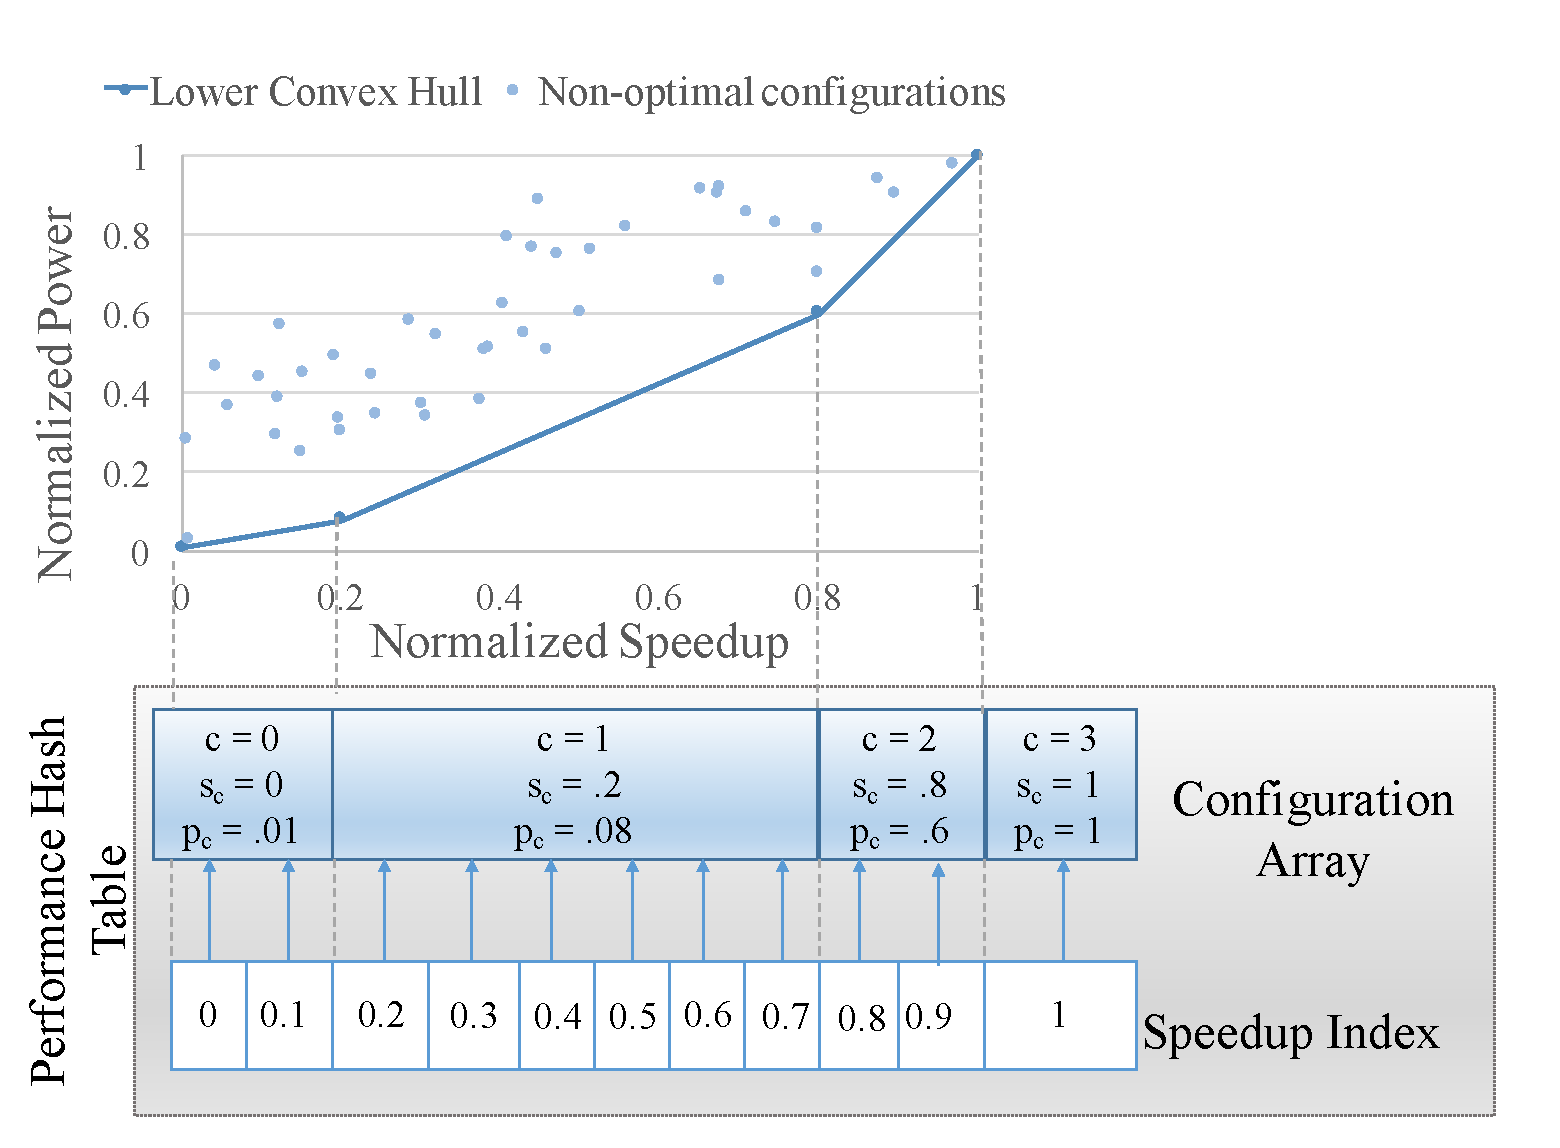
\includegraphics[width=\columnwidth]{figures/performance-hash-table.pdf}
\caption{Data structure to efficiently convert required speedup into a
  configuration.}
  \label{fig:pht}
\end{figure}

The PHT (illustrated in \figref{fig:pht}) only contains points on the
lower convex hull of the power/performance tradeoff space.  It
consists of two arrays: an array of pointers that point into a second
array, which stores the configurations on the convex hull sorted by
speedup.  Recall that speedups are computed relative to the base speed
which uses all resources.  We therefore know the largest speedup is 1,
so we need only concern ourselves with speedups less than 1.  The
first table, of pointers has a \emph{resolution} indicating how many
decimal points of precision it captures.  The example in
\figref{fig:pht} has a resolution of $0.1$.  Each pointer in the first
table points to the configuration in the second array that has the
largest speedup less than or equal to the index.

To use the table, the optimizer (\figref{fig:overview}) receives a
speedup $speedup(t)$ from the controller.  It converts this into two
configurations referred to as $hi$ and $lo$.  To find the $hi$
configuration, the translator clamps the desired speedup to the
largest index lower than $speedup(t)$ and then walks forward until it
finds the first configuration with a speedup higher than $speedup(t)$.
This configuration is $hi$.  To find the $lo$ configuration, the
translator clamps the desired speedup to the smallest index higher
than $speedup(t)$ and then walks backwards until it finds the
configuration with the largest speedup less than $speedup(t)$.

For example, consider the PHT in \figref{fig:pht} and an optimizer
meeting $speedup(t) = .65$.  To find $hi$, the optimizer indexes at .6
and walks up to find $c=2$ with $s_c=.8$, setting $hi = 2$.  To find
$lo$, the optimizer indexes the table at .7 and walks backward to find
$c=1$ with $s_c=.2$, setting $lo = 1$.

Finally, the optimizer sets $\tau_{hi}$ and $\tau_{lo}$ by solving the
following set of equations:
\begin{eqnarray}
  T &=& \tau_{hi} + \tau_{lo}    \label{eqn:s1} \\
  speedup(t) &=& \frac{s_{hi} \cdot \tau_{hi} + s_{lo} \cdot \tau_{lo}}{T} \label{eqn:s2}
\end{eqnarray}
In these equations, $speedup(t)$ is the speedup requested by the
controller and $s_c$ are speedups estimated by the learner.  By
solving \eqnsref{s1}{s2}, the optimizer has turned the controller's
speedup into a schedule of resource allocations using the models
provided by the HBM.

\PUNT{ Provided that the resolution is large enough to get a good
  spread of configurations to indices, the translator will always
  index the configuration array at most one entry from where it needs
  to be.  Thus, the entire translation process runs in constant time
  -- assuming that the learner is responsible for building the PHT
  once before passing it on to the translator.  This efficiency comes
  at a cost of memory usage -- many of the entries in the speedup
  index table will point to redundant locations in the configuration
  array.  We think that this is a reasonable tradeoff to make in
  practice as the code that runs on the mobile device must be fast or
  we risk wasting energy while trying to save energy.  In practice, we
  recommend a table of size 100 which provides a sufficient resolution
  and is not too wasteful of space.}


\subsection{Analysis}
%\subsubsection{Algorithmic Analysis}

\noindent \textbf{Control System Complexity} The GCS (see Algorithm
\ref{alg:gcs}) runs on the mobile or embedded device; each controller
invocation is $O(1)$ .  The only part that is not obviously constant
time is the PHT lookups.  Provided the PHT resolution is sufficiently
high to avoid collisions, then each PHT lookup requires constant time.
\begin{algorithm}[t]
\caption{Generalized control system}
\label{alg:gcs}
\begin{algorithmic}
\REQUIRE Initialize the controller with random configurations. Send power and performance samples to server and get performance hash table(PHT) from the server.
\WHILE{$True$}
    \STATE    Measure streaming application performance 
    \STATE    Compute required speedup (Equation \eqref{eqn:speedup})
    \STATE    Lookup $s_{hi}$ and $s_{lo}$ with PHT
    \STATE    Compute $\tau_{hi}$ and $\tau_{lo}$ (Equations \ref{eqn:s1} \& \ref{eqn:s2})
    \STATE    Configure to system to $hi$ $\&$ sleep $\tau_hi$.
    \STATE    Configure to $lo$ $\&$ sleep $\tau_lo$.
\ENDWHILE
\end{algorithmic}
\end{algorithm}


\noindent \textbf{Learning System Complexity} We run our learning
system on a remote server because the Hierarchical Bayesian Model
(HBM) is a relatively complex algorithm and it utilizes data from
other applications which can be stored in advance on the server
machines, allowing consolidation of data across similar devices.  The
time complexity for the HBM is $O(mn^3)$ where $m$ is the number of
applications and $n$ is the number of configurations.  Second step,
creating convex hull for the PHT takes $O(n log(n))$.

\subsection{Control Theoretic Formal Guarantees}
\label{sec:guarantees}
As mention above, the pole $p$ is critical to connecting the control
system of Equation \ref{eqn:speedup} to the HBM of Equation
\ref{eq:HBN}.  In \SYSTEM{}, we know the model variance $\sigma$ from
the HBM so we use that information to derive a lower bound for the
pole which guarantees probabilistic convergence to the desired
performance. Specifically, we prove that with probability 99.7\% the
system will converge to the desired performance if the pole is set to,
$$\Floor{1- \Floor{max(\hat{s})/(min(\hat{s}) - 3\sigma)}_0}_0 \leq p
\leq 1,$$ where $\Floor{x}_0 = \max(x,0)$ and $\hat{s}$ is the
estimated speedup. We include the proof of this claim in the appendix. In principle, users who need higher confidence
could set the scalar multiplier on $\sigma$ higher, using $6$ for
example provides a 99.99966\% probability of convergence.  

Thus we provide a lower-bound on the value of $p$ required for a
user to be confident that CALOREE will converge to the desired
performance.  This value for the pole only considers performance,
and not energy efficiency.  In practice, we find that it is
often better to use a higher pole based on the \emph{uncertainty}
between the controller's observed energy efficiency and that predicted
by the model.  We follow prior work in quantifying uncertainty as
$\rho$ \cite{Tokic2010}:
\begin{equation}
  \begin{array}{rcl}
    temp(t) &=& e^{\frac{- \left| (\frac{\bar{s}(t)}{\bar{p}(t)}  -\frac{ \hat{s}(t)}{\hat{p}_(t)} \right| }{5}} \\
    \rho(t) &=& \frac{1-temp(t)}{1+temp(t)} 
  \end{array}
  \label{eqn:uncer}
\end{equation}
where $\bar{s}$ and $\bar{p}$ are the measured values of speedup and
power up and $\hat{s}$ and $\hat{p}$ are the estimated values from the
HBM.  This measure of uncertainty captures both power and performance.
We find that it is generally higher than the pole value given by our
lower bound, so in practice we set the pole dynamically to be the
higher of the two values and we allow the GCS to make spot updates to
the estimated speedup and power based on its observations.  

\section{Experimental evaluations}


\begin{figure*}[t]
  \begin{tikzpicture}
\definecolor{s1}{RGB}{228, 26, 28}
\definecolor{s2}{RGB}{55, 126, 184}
\definecolor{s3}{RGB}{77, 175, 74}
\definecolor{s4}{RGB}{152, 78, 163}
\definecolor{s5}{RGB}{255, 127, 0}

\begin{groupplot}[
    group style={
        group name=plots,
        group size=1 by 1,
        xlabels at=edge top,
        xticklabels at=edge top,
        vertical sep=5pt
    },
axis x line* = top,
xlabel near ticks,
major x tick style = transparent,
height=3cm,
width=0.88\textwidth,
xmin=0,
xmax=9,
enlargelimits=false,
tick align = outside,
tick style={white},
ylabel style={align=center},
ytick=\empty,
xtick=\empty,
xticklabels={},
yticklabels={},
ymin=0,
ymax=1,
]
\nextgroupplot[ylabel={},
y label style={rotate=270},
ylabel shift={12mm},
]
\addplot[thick,solid, color=black] coordinates {(0,1) (22,1)};

\nextgroupplot[
ylabel shift={12mm},
y label style={rotate=270},
ylabel={$\mathsf{30\%}$},
]
\addplot[thick,solid, color=black] coordinates {(0,1) (22,1)};

\nextgroupplot[
ylabel shift={12mm},
y label style={rotate=270},
ylabel={$\mathsf{50\%}$},
]
\addplot[thick,solid, color=black] coordinates {(0,1) (22,1)};


\nextgroupplot[
ylabel shift={12mm},
ylabel={$\mathsf{70\%}$},
y label style={rotate=270},
]
\addplot[thick,solid, color=black] coordinates {(0,1) (22,1)};

\nextgroupplot[
ylabel shift={12mm},
ylabel={$\mathsf{90\%}$},
y label style={rotate=270},
]
\addplot[thick,solid, color=black] coordinates {(0,1) (22,1)};

\end{groupplot}

\begin{groupplot}[
    group style={
        group name=plots,
        group size=1 by 2,
        xlabels at=edge bottom,
        xticklabels at=edge bottom,
        vertical sep=5pt
    },
axis x line* = bottom,
xlabel near ticks,
major x tick style = transparent,
xlabel={},
height=3cm,
width=0.88\textwidth,
xmin=0,
xmax=22,
enlargelimits=false,
tick align = outside,
tick style={white},
ylabel style={align=center},
ytick=\empty,
ymin=0,
ymax=1.1,
ytick={0,0.3,0.6,0.9},
yticklabels={,0.3,0.6,0.9},
legend cell align=left, 
legend style={ column sep=1ex },
ymajorgrids,
grid style={dashed},
]


\nextgroupplot[ybar=\pgflinewidth,
bar width=2.0pt,
legend entries = {{$\mathsf{Online}$},{$\mathsf{Offline}$},{$\mathsf{LEO}$}},
legend style={draw=none,legend columns=3,at={(.5,1.7)},anchor=north},
ylabel={\footnotesize Accuracy\\ (Performance)}, 
ylabel shift={0mm},
]
\addplot table[x index=0,y index=5, col sep=space] {img/image_text/accuracy.txt};
\addplot table[x index=0,y index=7, col sep=space] {img/image_text/accuracy.txt};
\addplot table[x index=0,y index=3, col sep=space] {img/image_text/accuracy.txt};

\nextgroupplot[ybar=\pgflinewidth,
bar width=2.0pt,
ylabel={\footnotesize Accuracy\\ (Power)}, 
ylabel shift={0mm},
xticklabel shift={0pt},
x tick label style={rotate=35, anchor=east},
xtick={1,2,3,4,5,6,7,8,9,10,11,12,13,14,15,16,17,18,19,20,21,22},
xticklabels={
{\scriptsize $\mathsf{backprop}$},
{\scriptsize $\mathsf{bfs}$},
{\scriptsize $\mathsf{blackscholes}$},
{\scriptsize $\mathsf{bodytrack}$},
{\scriptsize $\mathsf{facesim}$},
{\scriptsize $\mathsf{ferret}$},
{\scriptsize $\mathsf{heartwall}$},
{\scriptsize $\mathsf{hotspot}$},
{\scriptsize $\mathsf{jacobi}$},
{\scriptsize $\mathsf{kmeans}$},
{\scriptsize $\mathsf{kmeansnf}$},
{\scriptsize $\mathsf{lavamd}$},
{\scriptsize $\mathsf{leukocyte}$},
{\scriptsize $\mathsf{lud}$},
{\scriptsize $\mathsf{nw}$},
{\scriptsize $\mathsf{sha}$},
{\scriptsize $\mathsf{srad}$},
{\scriptsize $\mathsf{stream_threads}$},
{\scriptsize $\mathsf{x264-ducks}$},
{\scriptsize $\mathsf{x264-native}$},
{\scriptsize $\mathsf{\mathbf{Average}}$}},
]
\addplot table[x index=0,y index=4, col sep=space] {img/image_text/accuracy.txt};
\addplot table[x index=0,y index=6, col sep=space] {img/image_text/accuracy.txt};
\addplot table[x index=0,y index=2, col sep=space] {img/image_text/accuracy.txt};

\end{groupplot}
\end{tikzpicture}
   \vskip -1em
  \caption{Accuracy performance}
  \label{fig:accuracy}
\end{figure*}


\begin{figure*}[t]
  \begin{tikzpicture}
\definecolor{s1}{RGB}{228, 26, 28}
\definecolor{s2}{RGB}{55, 126, 184}
\definecolor{s3}{RGB}{77, 175, 74}
\definecolor{s4}{RGB}{152, 78, 163}
\definecolor{s5}{RGB}{255, 127, 0}

\begin{groupplot}[
    group style={
        group name=plots,
        group size=1 by 1,
        xlabels at=edge top,
        xticklabels at=edge top,
        vertical sep=5pt
    },
axis x line* = top,
xlabel near ticks,
major x tick style = transparent,
height=2.5cm,
width=0.88\textwidth,
xmin=0,
xmax=9,
enlargelimits=false,
tick align = outside,
tick style={white},
ylabel style={align=center},
ytick=\empty,
xtick=\empty,
xticklabels={},
yticklabels={},
ymin=0,
ymax=1,
]
\nextgroupplot[ylabel={},
y label style={rotate=270},
ylabel shift={12mm},
]
\addplot[thick,solid, color=black] coordinates {(0,1) (22,1)};

\nextgroupplot[
ylabel shift={12mm},
y label style={rotate=270},
ylabel={$\mathsf{30\%}$},
]
\addplot[thick,solid, color=black] coordinates {(0,1) (22,1)};

\nextgroupplot[
ylabel shift={12mm},
y label style={rotate=270},
ylabel={$\mathsf{50\%}$},
]
\addplot[thick,solid, color=black] coordinates {(0,1) (22,1)};


\nextgroupplot[
ylabel shift={12mm},
ylabel={$\mathsf{70\%}$},
y label style={rotate=270},
]
\addplot[thick,solid, color=black] coordinates {(0,1) (22,1)};

\nextgroupplot[
ylabel shift={12mm},
ylabel={$\mathsf{90\%}$},
y label style={rotate=270},
]
\addplot[thick,solid, color=black] coordinates {(0,1) (22,1)};

\end{groupplot}

\begin{groupplot}[
    group style={
        group name=plots,
        group size=1 by 3,
        xlabels at=edge bottom,
        xticklabels at=edge bottom,
        vertical sep=5pt
    },
axis x line* = bottom,
xlabel near ticks,
major x tick style = transparent,
xlabel={},
height=2.5cm,
width=0.88\textwidth,
xmin=0,
xmax=22,
enlargelimits=false,
tick align = outside,
tick style={white},
ylabel style={align=center},
ytick=\empty,
ymin=0,
ymax=1,
ytick={0,0.5,1.0},
yticklabels={0,0.75,1.0},
legend cell align=left, 
legend style={ column sep=1ex },
ymajorgrids,
grid style={dashed},
]



\nextgroupplot[ybar=\pgflinewidth,
bar width=2.0pt,
legend entries = {{$\mathsf{Online}$},{$\mathsf{Offline}$},{$\mathsf{LEO}$}},
legend style={draw=none,legend columns=3,at={(.5,1.7)},anchor=north},
ylabel shift={0mm},
xticklabel shift={0pt},
x tick label style={rotate=35, anchor=east},
xtick={1,2,3,4,5,6,7,8,9,10,11,12,13,14,15,16,17,18,19,20,21,22},
xticklabels={
{\scriptsize $\mathsf{backprop}$},
{\scriptsize $\mathsf{bfs}$},
{\scriptsize $\mathsf{blackscholes}$},
{\scriptsize $\mathsf{bodytrack}$},
{\scriptsize $\mathsf{facesim}$},
{\scriptsize $\mathsf{ferret}$},
{\scriptsize $\mathsf{heartwall}$},
{\scriptsize $\mathsf{hotspot}$},
{\scriptsize $\mathsf{jacobi}$},
{\scriptsize $\mathsf{kmeans}$},
{\scriptsize $\mathsf{kmeansnf}$},
{\scriptsize $\mathsf{lavamd}$},
{\scriptsize $\mathsf{leukocyte}$},
{\scriptsize $\mathsf{lud}$},
{\scriptsize $\mathsf{nw}$},
{\scriptsize $\mathsf{sha}$},
{\scriptsize $\mathsf{srad}$},
{\scriptsize $\mathsf{stream_threads}$},
{\scriptsize $\mathsf{x264-ducks}$},
{\scriptsize $\mathsf{x264-native}$},
{\scriptsize $\mathsf{\mathbf{Average}}$}},
]
\addplot table[x index=0,y index=5, col sep=space] {img/image_text/accuracy.txt};
\addplot table[x index=0,y index=7, col sep=space] {img/image_text/accuracy.txt};
\addplot table[x index=0,y index=3, col sep=space] {img/image_text/accuracy.txt};

\end{groupplot}
\end{tikzpicture}
   \vskip -1em
  \caption{Accuracy power}
  \label{fig:accuracy}
\end{figure*}

\begin{figure*}[t]
  \begin{tikzpicture}
\definecolor{s1}{RGB}{228, 26, 28}
\definecolor{s2}{RGB}{55, 126, 184}
\definecolor{s3}{RGB}{77, 175, 74}
\definecolor{s4}{RGB}{152, 78, 163}
\definecolor{s5}{RGB}{255, 127, 0}

\begin{groupplot}[
    group style={
        group name=plots,
        group size=1 by 5,
        xlabels at=edge top,
        xticklabels at=edge top,
        vertical sep=5pt
    },
axis x line* = top,
xlabel near ticks,
major x tick style = transparent,
height=2.5cm,
width=0.88\textwidth,
xmin=0,
xmax=9,
enlargelimits=false,
tick align = outside,
tick style={white},
ylabel style={align=center},
ytick=\empty,
xtick=\empty,
xticklabels={},
yticklabels={},
ymin=0,
ymax=1,
]
\nextgroupplot[ylabel={$\mathsf{10\%}$},
y label style={rotate=270},
ylabel shift={12mm},
]
\addplot[thick,solid, color=black] coordinates {(0,1) (22,1)};

\nextgroupplot[
ylabel shift={12mm},
y label style={rotate=270},
ylabel={$\mathsf{30\%}$},
]
\addplot[thick,solid, color=black] coordinates {(0,1) (22,1)};

\nextgroupplot[
ylabel shift={12mm},
y label style={rotate=270},
ylabel={$\mathsf{50\%}$},
]
\addplot[thick,solid, color=black] coordinates {(0,1) (22,1)};


\nextgroupplot[
ylabel shift={12mm},
ylabel={$\mathsf{70\%}$},
y label style={rotate=270},
]
\addplot[thick,solid, color=black] coordinates {(0,1) (22,1)};

\nextgroupplot[
ylabel shift={12mm},
ylabel={$\mathsf{90\%}$},
y label style={rotate=270},
]
\addplot[thick,solid, color=black] coordinates {(0,1) (22,1)};

\end{groupplot}

\begin{groupplot}[
    group style={
        group name=plots,
        group size=1 by 5,
        xlabels at=edge bottom,
        xticklabels at=edge bottom,
        vertical sep=5pt
    },
axis x line* = bottom,
xlabel near ticks,
major x tick style = transparent,
xlabel={},
height=2.5cm,
width=0.88\textwidth,
xmin=0,
xmax=22,
enlargelimits=false,
tick align = outside,
tick style={white},
ylabel style={align=center},
ytick=\empty,
ymin=0,
ymax=30,
ytick={0,5,10,15,20},
yticklabels={,5,10,15,20},
legend cell align=left, 
legend style={ column sep=1ex },
ymajorgrids,
grid style={dashed},
]

\nextgroupplot[ybar=\pgflinewidth,
bar width=2.0pt,
legend entries = {{$\mathsf{Online-P2I}$},{$\mathsf{Offline-P2I}$},{$\mathsf{LEO-P2I}$},{$\mathsf{POET}$},{$\mathsf{\SYSTEM{}}$}},
legend style={draw=none,legend columns=5,at={(.5,1.7)},anchor=north},
ylabel shift={0mm},
ymin=0,
ymax=6,
ytick={0.0,2.0,4.0,6.0},
yticklabels={,2.0,4.0,6.0},
]
\addplot table[x index=0,y index=3, col sep=space] {img/image_text/dyn-mape-0.1.txt};
\addplot table[x index=0,y index=4, col sep=space] {img/image_text/dyn-mape-0.1.txt};
\addplot table[x index=0,y index=5, col sep=space] {img/image_text/dyn-mape-0.1.txt};
\addplot table[x index=0,y index=6, col sep=space] {img/image_text/dyn-mape-0.1.txt};
\addplot table[x index=0,y index=7, col sep=space] {img/image_text/dyn-mape-0.1.txt};

\nextgroupplot[ybar=\pgflinewidth,
ylabel shift={0mm},
bar width=2.0pt,
ymin=0,
ymax=20,
ytick={0.0,5.0,10.0,15.0,20.0},
yticklabels={,5.0,10.0,15.0},
]
\addplot table[x index=0,y index=3, col sep=space] {img/image_text/dyn-mape-0.3.txt};
\addplot table[x index=0,y index=4, col sep=space] {img/image_text/dyn-mape-0.3.txt};
\addplot table[x index=0,y index=5, col sep=space] {img/image_text/dyn-mape-0.3.txt};
\addplot table[x index=0,y index=6, col sep=space] {img/image_text/dyn-mape-0.3.txt};
\addplot table[x index=0,y index=7, col sep=space] {img/image_text/dyn-mape-0.3.txt};

\nextgroupplot[ybar=\pgflinewidth,
ylabel={\footnotesize MAPE},
ylabel shift={0mm},
bar width=2.0pt,
ymin=0,
ymax=30,
ytick={0.0,10.0,20.0,30.0},
yticklabels={,10.0,20.0,30.0},
]
\addplot table[x index=0,y index=3, col sep=space] {img/image_text/dyn-mape-0.5.txt};
\addplot table[x index=0,y index=4, col sep=space] {img/image_text/dyn-mape-0.5.txt};
\addplot table[x index=0,y index=5, col sep=space] {img/image_text/dyn-mape-0.5.txt};
\addplot table[x index=0,y index=6, col sep=space] {img/image_text/dyn-mape-0.5.txt};
\addplot table[x index=0,y index=7, col sep=space] {img/image_text/dyn-mape-0.5.txt};

\nextgroupplot[ybar=\pgflinewidth,
ylabel shift={0mm},
bar width=2.0pt,
ymin=0,
ymax=30,
ytick={0.0,10.0,20.0,30.0},
yticklabels={,10.0,20.0,30.0},
]
\addplot table[x index=0,y index=3, col sep=space] {img/image_text/dyn-mape-0.7.txt};
\addplot table[x index=0,y index=4, col sep=space] {img/image_text/dyn-mape-0.7.txt};
\addplot table[x index=0,y index=5, col sep=space] {img/image_text/dyn-mape-0.7.txt};
\addplot table[x index=0,y index=6, col sep=space] {img/image_text/dyn-mape-0.7.txt};
\addplot table[x index=0,y index=7, col sep=space] {img/image_text/dyn-mape-0.7.txt};

\nextgroupplot[ybar=\pgflinewidth,
bar width=2.0pt,
ylabel shift={0mm},
xticklabel shift={0pt},
ymin=0,
ymax=30,
ytick={0.0,10.0,20.0,30.0},
yticklabels={,10.0,20.0,30.0},
x tick label style={rotate=35, anchor=east},
xtick={1,2,3,4,5,6,7,8,9,10,11,12,13,14,15,16,17,18,19,20,21,22},
xticklabels={
{\scriptsize $\mathsf{backprop}$},
{\scriptsize $\mathsf{bfs}$},
{\scriptsize $\mathsf{blackscholes}$},
{\scriptsize $\mathsf{bodytrack}$},
{\scriptsize $\mathsf{facesim}$},
{\scriptsize $\mathsf{ferret}$},
{\scriptsize $\mathsf{heartwall}$},
{\scriptsize $\mathsf{hotspot}$},
{\scriptsize $\mathsf{jacobi}$},
{\scriptsize $\mathsf{kmeans}$},
{\scriptsize $\mathsf{kmeansnf}$},
{\scriptsize $\mathsf{lavamd}$},
{\scriptsize $\mathsf{leukocyte}$},
{\scriptsize $\mathsf{lud}$},
{\scriptsize $\mathsf{nw}$},
{\scriptsize $\mathsf{sha}$},
{\scriptsize $\mathsf{srad}$},
{\scriptsize $\mathsf{stream_threads}$},
{\scriptsize $\mathsf{x264-ducks}$},
{\scriptsize $\mathsf{x264-native}$},
{\scriptsize $\mathsf{\mathbf{Average}}$}},
]
\addplot table[x index=0,y index=3, col sep=space] {img/image_text/dyn-mape-0.9.txt};
\addplot table[x index=0,y index=4, col sep=space] {img/image_text/dyn-mape-0.9.txt};
\addplot table[x index=0,y index=5, col sep=space] {img/image_text/dyn-mape-0.9.txt};
\addplot table[x index=0,y index=6, col sep=space] {img/image_text/dyn-mape-0.9.txt};
\addplot table[x index=0,y index=7, col sep=space] {img/image_text/dyn-mape-0.9.txt};

\end{groupplot}
\end{tikzpicture}
   \vskip -1em
  \caption{Single Applications MAPE}
  \label{fig:single-perf}
\end{figure*}

\begin{figure*}[t]
  \begin{tikzpicture}
\definecolor{s1}{RGB}{228, 26, 28}
\definecolor{s2}{RGB}{55, 126, 184}
\definecolor{s3}{RGB}{77, 175, 74}
\definecolor{s4}{RGB}{152, 78, 163}
\definecolor{s5}{RGB}{255, 127, 0}

\begin{groupplot}[
    group style={
        group name=plots,
        group size=1 by 5,
        xlabels at=edge top,
        xticklabels at=edge top,
        vertical sep=5pt
    },
axis x line* = top,
xlabel near ticks,
major x tick style = transparent,
height=2.5cm,
width=0.88\textwidth,
xmin=0,
xmax=9,
enlargelimits=false,
tick align = outside,
tick style={white},
ylabel style={align=center},
ytick=\empty,
xtick=\empty,
xticklabels={},
yticklabels={},
ymin=0,
ymax=1,
]
\nextgroupplot[ylabel={$\mathsf{10\%}$},
y label style={rotate=270},
ylabel shift={12mm},
]
\addplot[thick,solid, color=black] coordinates {(0,1) (22,1)};
\nextgroupplot[
ylabel shift={12mm},
y label style={rotate=270},
ylabel={$\mathsf{30\%}$},
]
\addplot[thick,solid, color=black] coordinates {(0,1) (22,1)};
\nextgroupplot[
ylabel shift={12mm},
y label style={rotate=270},
ylabel={$\mathsf{50\%}$},
]
\addplot[thick,solid, color=black] coordinates {(0,1) (22,1)};
\nextgroupplot[
ylabel shift={12mm},
ylabel={$\mathsf{70\%}$},
y label style={rotate=270},
]
\addplot[thick,solid, color=black] coordinates {(0,1) (22,1)};
\nextgroupplot[
ylabel shift={12mm},
ylabel={$\mathsf{90\%}$},
y label style={rotate=270},
]
\addplot[thick,solid, color=black] coordinates {(0,1) (22,1)};
\end{groupplot}

\begin{groupplot}[
    group style={
        group name=plots,
        group size=1 by 5,
        xlabels at=edge bottom,
        xticklabels at=edge bottom,
        vertical sep=5pt
    },
axis x line* = bottom,
xlabel near ticks,
major x tick style = transparent,
xlabel={},
height=2.5cm,
width=0.88\textwidth,
xmin=0,
xmax=22,
enlargelimits=false,
tick align = outside,
tick style={white},
ylabel style={align=center},
ytick=\empty,
ymin=0,
ymax=2.5,
ytick={0,0.50,1.50,2.50},
yticklabels={,50,150,250},
legend cell align=left, 
legend style={ column sep=1ex },
ymajorgrids,
grid style={dashed},
]

\nextgroupplot[ybar=\pgflinewidth,
bar width=2.0pt,
legend entries = {{$\mathsf{Online-P2I}$},{$\mathsf{Offline-P2I}$},{$\mathsf{LEO-P2I}$},{$\mathsf{POET}$},{$\mathsf{\SYSTEM{}}$}},
legend style={draw=none,legend columns=5,at={(.5,1.7)},anchor=north},
ylabel shift={0mm},
ymin=0,
ymax=2,
ytick={0,0.5,1.5,2},
yticklabels={,50,150,200},
]
\addplot table[x index=0,y index=3, col sep=space] {img/image_text/dyn-eff-0.1.txt};
\addplot table[x index=0,y index=4, col sep=space] {img/image_text/dyn-eff-0.1.txt};
\addplot table[x index=0,y index=5, col sep=space] {img/image_text/dyn-eff-0.1.txt};
\addplot table[x index=0,y index=6, col sep=space] {img/image_text/dyn-eff-0.1.txt};
\addplot table[x index=0,y index=7, col sep=space] {img/image_text/dyn-eff-0.1.txt};

\nextgroupplot[ybar=\pgflinewidth,
ylabel shift={0mm},
bar width=2.0pt,
%ymin=.9,
%ymax=9,
%ytick={1,2,3,4,5,6,7,8},
%yticklabels={1.0,,,,5.0,,,8.0},
]
\addplot table[x index=0,y index=3, col sep=space] {img/image_text/dyn-eff-0.3.txt};
\addplot table[x index=0,y index=4, col sep=space] {img/image_text/dyn-eff-0.3.txt};
\addplot table[x index=0,y index=5, col sep=space] {img/image_text/dyn-eff-0.3.txt};
\addplot table[x index=0,y index=6, col sep=space] {img/image_text/dyn-eff-0.3.txt};
\addplot table[x index=0,y index=7, col sep=space] {img/image_text/dyn-eff-0.3.txt};

\nextgroupplot[ybar=\pgflinewidth,
ylabel={\footnotesize Normalized energy},
ylabel shift={0mm},
bar width=2.0pt,
%ymin=.9,
%ymax=9,
%ytick={1,2,3,4,5,6,7,8},
%yticklabels={1.0,,,,5.0,,,8.0},
]
\addplot table[x index=0,y index=3, col sep=space] {img/image_text/dyn-eff-0.5.txt};
\addplot table[x index=0,y index=4, col sep=space] {img/image_text/dyn-eff-0.5.txt};
\addplot table[x index=0,y index=5, col sep=space] {img/image_text/dyn-eff-0.5.txt};
\addplot table[x index=0,y index=6, col sep=space] {img/image_text/dyn-eff-0.5.txt};
\addplot table[x index=0,y index=7, col sep=space] {img/image_text/dyn-eff-0.5.txt};

\nextgroupplot[ybar=\pgflinewidth,
ylabel shift={0mm},
bar width=2.0pt,
%ymin=.9,
%ymax=9,
%ytick={1,2,3,4,5,6,7,8},
%yticklabels={1.0,,,,5.0,,,8.0},
ymin=0,
ymax=3,
ytick={0,1,2,3},
yticklabels={,100,200,300},
]
\addplot table[x index=0,y index=3, col sep=space] {img/image_text/dyn-eff-0.7.txt};
\addplot table[x index=0,y index=4, col sep=space] {img/image_text/dyn-eff-0.7.txt};
\addplot table[x index=0,y index=5, col sep=space] {img/image_text/dyn-eff-0.7.txt};
\addplot table[x index=0,y index=6, col sep=space] {img/image_text/dyn-eff-0.7.txt};
\addplot table[x index=0,y index=7, col sep=space] {img/image_text/dyn-eff-0.7.txt};

\nextgroupplot[ybar=\pgflinewidth,
bar width=2.0pt,
ylabel shift={0mm},
xticklabel shift={0pt},
x tick label style={rotate=35, anchor=east},
xtick={1,2,3,4,5,6,7,8,9,10,11,12,13,14,15,16,17,18,19,20,21,22},
ymin=0,
ymax=3.1,
ytick={0,1,2,3},
yticklabels={,100,200,300},
xticklabels={
{\scriptsize $\mathsf{backprop}$},
{\scriptsize $\mathsf{bfs}$},
{\scriptsize $\mathsf{blackscholes}$},
{\scriptsize $\mathsf{bodytrack}$},
{\scriptsize $\mathsf{facesim}$},
{\scriptsize $\mathsf{ferret}$},
{\scriptsize $\mathsf{heartwall}$},
{\scriptsize $\mathsf{hotspot}$},
{\scriptsize $\mathsf{jacobi}$},
{\scriptsize $\mathsf{kmeans}$},
{\scriptsize $\mathsf{kmeansnf}$},
{\scriptsize $\mathsf{lavamd}$},
{\scriptsize $\mathsf{leukocyte}$},
{\scriptsize $\mathsf{lud}$},
{\scriptsize $\mathsf{nw}$},
{\scriptsize $\mathsf{sha}$},
{\scriptsize $\mathsf{srad}$},
{\scriptsize $\mathsf{stream_threads}$},
{\scriptsize $\mathsf{x264-ducks}$},
{\scriptsize $\mathsf{x264-native}$},
{\scriptsize $\mathsf{\mathbf{Average}}$}},
]
\addplot table[x index=0,y index=3, col sep=space] {img/image_text/dyn-eff-0.9.txt};
\addplot table[x index=0,y index=4, col sep=space] {img/image_text/dyn-eff-0.9.txt};
\addplot table[x index=0,y index=5, col sep=space] {img/image_text/dyn-eff-0.9.txt};
\addplot table[x index=0,y index=6, col sep=space] {img/image_text/dyn-eff-0.9.txt};
\addplot table[x index=0,y index=7, col sep=space] {img/image_text/dyn-eff-0.9.txt};

\end{groupplot}
\end{tikzpicture}
   \vskip -1em
  \caption{Single Applications energy}
  \label{fig:single-energy}
\end{figure*}


\begin{figure*}[t]
  \begin{tikzpicture}
\definecolor{s1}{RGB}{228, 26, 28}
\definecolor{s2}{RGB}{55, 126, 184}
\definecolor{s3}{RGB}{77, 175, 74}
\definecolor{s4}{RGB}{152, 78, 163}
\definecolor{s5}{RGB}{255, 127, 0}

\begin{groupplot}[
    group style={
        group name=plots,
        group size=1 by 5,
        xlabels at=edge top,
        xticklabels at=edge top,
        vertical sep=5pt
    },
axis x line* = top,
xlabel near ticks,
major x tick style = transparent,
height=2.5cm,
width=0.88\textwidth,
xmin=0,
xmax=9,
enlargelimits=false,
tick align = outside,
tick style={white},
ylabel style={align=center},
ytick=\empty,
xtick=\empty,
xticklabels={},
yticklabels={},
ymin=0,
ymax=1,
]
\nextgroupplot[ylabel={$\mathsf{10\%}$},
y label style={rotate=270},
ylabel shift={12mm},
]
\addplot[thick,solid, color=black] coordinates {(0,1) (22,1)};

\nextgroupplot[
ylabel shift={12mm},
y label style={rotate=270},
ylabel={$\mathsf{30\%}$},
]
\addplot[thick,solid, color=black] coordinates {(0,1) (22,1)};

\nextgroupplot[
ylabel shift={12mm},
y label style={rotate=270},
ylabel={$\mathsf{50\%}$},
]
\addplot[thick,solid, color=black] coordinates {(0,1) (22,1)};


\nextgroupplot[
ylabel shift={12mm},
ylabel={$\mathsf{70\%}$},
y label style={rotate=270},
]
\addplot[thick,solid, color=black] coordinates {(0,1) (22,1)};

\nextgroupplot[
ylabel shift={12mm},
ylabel={$\mathsf{90\%}$},
y label style={rotate=270},
]
\addplot[thick,solid, color=black] coordinates {(0,1) (22,1)};

\end{groupplot}

\begin{groupplot}[
    group style={
        group name=plots,
        group size=1 by 5,
        xlabels at=edge bottom,
        xticklabels at=edge bottom,
        vertical sep=5pt
    },
axis x line* = bottom,
xlabel near ticks,
major x tick style = transparent,
xlabel={},
height=2.5cm,
width=0.88\textwidth,
xmin=0,
xmax=22,
enlargelimits=false,
tick align = outside,
tick style={white},
ylabel style={align=center},
ytick=\empty,
ymin=0,
ymax=35,
ytick={0,5,15,25,35},
yticklabels={,5,15,25,35},
legend cell align=left, 
legend style={ column sep=1ex },
ymajorgrids,
grid style={dashed},
]

\nextgroupplot[ybar=\pgflinewidth,
bar width=2.0pt,
legend entries = {{$\mathsf{Online-P2I}$},{$\mathsf{Offline-P2I}$},{$\mathsf{LEO-P2I}$},{$\mathsf{POET}$},{$\mathsf{\SYSTEM{}}$}},
legend style={draw=none,legend columns=5,at={(.5,1.7)},anchor=north},
ylabel shift={0mm},
]
\addplot table[x index=0,y index=2, col sep=space] {img/image_text/ma-err-0.1.txt};
\addplot table[x index=0,y index=3, col sep=space] {img/image_text/ma-err-0.1.txt};
\addplot table[x index=0,y index=4, col sep=space] {img/image_text/ma-err-0.1.txt};
\addplot table[x index=0,y index=5, col sep=space] {img/image_text/ma-err-0.1.txt};
\addplot table[x index=0,y index=6, col sep=space] {img/image_text/ma-err-0.1.txt};

\nextgroupplot[ybar=\pgflinewidth,
ylabel shift={0mm},
bar width=2.0pt,
%ymin=.9,
%ymax=9,
%ytick={1,2,3,4,5,6,7,8},
%yticklabels={1.0,,,,5.0,,,8.0},
]
\addplot table[x index=0,y index=2, col sep=space] {img/image_text/ma-err-0.3.txt};
\addplot table[x index=0,y index=3, col sep=space] {img/image_text/ma-err-0.3.txt};
\addplot table[x index=0,y index=4, col sep=space] {img/image_text/ma-err-0.3.txt};
\addplot table[x index=0,y index=5, col sep=space] {img/image_text/ma-err-0.3.txt};
\addplot table[x index=0,y index=6, col sep=space] {img/image_text/ma-err-0.3.txt};

\nextgroupplot[ybar=\pgflinewidth,
ylabel={\footnotesize MAPE},
ylabel shift={0mm},
bar width=2.0pt,
%ymin=.9,
%ymax=9,
%ytick={1,2,3,4,5,6,7,8},
%yticklabels={1.0,,,,5.0,,,8.0},
]
\addplot table[x index=0,y index=2, col sep=space] {img/image_text/ma-err-0.5.txt};
\addplot table[x index=0,y index=3, col sep=space] {img/image_text/ma-err-0.5.txt};
\addplot table[x index=0,y index=4, col sep=space] {img/image_text/ma-err-0.5.txt};
\addplot table[x index=0,y index=5, col sep=space] {img/image_text/ma-err-0.5.txt};
\addplot table[x index=0,y index=6, col sep=space] {img/image_text/ma-err-0.5.txt};

\nextgroupplot[ybar=\pgflinewidth,
ylabel shift={0mm},
bar width=2.0pt,
%ymin=.9,
%ymax=9,
%ytick={1,2,3,4,5,6,7,8},
%yticklabels={1.0,,,,5.0,,,8.0},
]
\addplot table[x index=0,y index=2, col sep=space] {img/image_text/ma-err-0.7.txt};
\addplot table[x index=0,y index=3, col sep=space] {img/image_text/ma-err-0.7.txt};
\addplot table[x index=0,y index=4, col sep=space] {img/image_text/ma-err-0.7.txt};
\addplot table[x index=0,y index=5, col sep=space] {img/image_text/ma-err-0.7.txt};
\addplot table[x index=0,y index=6, col sep=space] {img/image_text/ma-err-0.7.txt};

\nextgroupplot[ybar=\pgflinewidth,
bar width=2.0pt,
ylabel shift={0mm},
xticklabel shift={0pt},
x tick label style={rotate=35, anchor=east},
xtick={1,2,3,4,5,6,7,8,9,10,11,12,13,14,15,16,17,18,19,20,21,22},
xticklabels={
{\scriptsize $\mathsf{backprop}$},
{\scriptsize $\mathsf{bfs}$},
{\scriptsize $\mathsf{blackscholes}$},
{\scriptsize $\mathsf{bodytrack}$},
{\scriptsize $\mathsf{facesim}$},
{\scriptsize $\mathsf{ferret}$},
{\scriptsize $\mathsf{heartwall}$},
{\scriptsize $\mathsf{hotspot}$},
{\scriptsize $\mathsf{jacobi}$},
{\scriptsize $\mathsf{kmeans}$},
{\scriptsize $\mathsf{kmeansnf}$},
{\scriptsize $\mathsf{lavamd}$},
{\scriptsize $\mathsf{leukocyte}$},
{\scriptsize $\mathsf{lud}$},
{\scriptsize $\mathsf{nw}$},
{\scriptsize $\mathsf{sha}$},
{\scriptsize $\mathsf{srad}$},
{\scriptsize $\mathsf{stream_threads}$},
{\scriptsize $\mathsf{x264-ducks}$},
{\scriptsize $\mathsf{x264-native}$},
{\scriptsize $\mathsf{\mathbf{Average}}$}},
]
\addplot table[x index=0,y index=2, col sep=space] {img/image_text/ma-err-0.9.txt};
\addplot table[x index=0,y index=3, col sep=space] {img/image_text/ma-err-0.9.txt};
\addplot table[x index=0,y index=4, col sep=space] {img/image_text/ma-err-0.9.txt};
\addplot table[x index=0,y index=5, col sep=space] {img/image_text/ma-err-0.9.txt};
\addplot table[x index=0,y index=6, col sep=space] {img/image_text/ma-err-0.9.txt};

\end{groupplot}
\end{tikzpicture}
   \vskip -1em
  \caption{Multi Applications MAPE}
  \label{fig:multi-perf}
\end{figure*}

\begin{figure*}[t]
  \begin{tikzpicture}
\definecolor{s1}{RGB}{228, 26, 28}
\definecolor{s2}{RGB}{55, 126, 184}
\definecolor{s3}{RGB}{77, 175, 74}
\definecolor{s4}{RGB}{152, 78, 163}
\definecolor{s5}{RGB}{255, 127, 0}
\definecolor{s6}{RGB}{239, 159, 0}
\definecolor{s7}{RGB}{86, 180, 233}

\begin{groupplot}[
    group style={
        group name=plots,
        group size=1 by 6,
        xlabels at=edge top,
        xticklabels at=edge top,
        vertical sep=5pt
    },
axis x line* = top,
xlabel near ticks,
major x tick style = transparent,
height=2.5cm,
width=0.88\textwidth,
xmin=0,
xmax=9,
enlargelimits=false,
tick align = outside,
tick style={white},
ylabel style={align=center},
ytick=\empty,
xtick=\empty,
xticklabels={},
yticklabels={},
ymin=0,
ymax=1,
]
\nextgroupplot[ylabel={$\mathsf{40\%}$},
y label style={rotate=270},
ylabel shift={12mm},
]
\addplot[thick,solid, color=black] coordinates {(0,1) (22,1)};

\nextgroupplot[
ylabel shift={12mm},
y label style={rotate=270},
ylabel={$\mathsf{50\%}$},
]
\addplot[thick,solid, color=black] coordinates {(0,1) (22,1)};

\nextgroupplot[
ylabel shift={12mm},
y label style={rotate=270},
ylabel={$\mathsf{60\%}$},
]
\addplot[thick,solid, color=black] coordinates {(0,1) (22,1)};


\nextgroupplot[
ylabel shift={12mm},
ylabel={$\mathsf{70\%}$},
y label style={rotate=270},
]
\addplot[thick,solid, color=black] coordinates {(0,1) (22,1)};

\nextgroupplot[
ylabel shift={12mm},
ylabel={$\mathsf{80\%}$},
y label style={rotate=270},
]
\addplot[thick,solid, color=black] coordinates {(0,1) (22,1)};

\nextgroupplot[
ylabel shift={12mm},
ylabel={$\mathsf{90\%}$},
y label style={rotate=270},
]
\addplot[thick,solid, color=black] coordinates {(0,1) (22,1)};

\end{groupplot}

\begin{groupplot}[
    group style={
        group name=plots,
        group size=1 by 6,
        xlabels at=edge bottom,
        xticklabels at=edge bottom,
        vertical sep=5pt
    },
axis x line* = bottom,
xlabel near ticks,
major x tick style = transparent,
xlabel={},
height=2.5cm,
width=0.88\textwidth,
xmin=0,
xmax=23,
enlargelimits=false,
tick align = outside,
tick style={white},
ylabel style={align=center},
ytick=\empty,
ymin=0.0,
ymax=45.0,
ytick={0.0,15.0,30.0,45.0},
yticklabels={,15.0,30.0,45.0},
legend cell align=left, 
legend style={ column sep=1ex },
ymajorgrids,
grid style={dashed},
]

\nextgroupplot[ybar=\pgflinewidth,
bar width=2.0pt,
legend entries = {{$\mathsf{Online}$},{$\mathsf{Offline}$},{$\mathsf{LEO}$},{$\mathsf{POET}$},{$\mathsf{\SYSTEM{}-NP}$},{$\mathsf{\SYSTEM{}}$}},
legend style={draw=none,legend columns=6,at={(.5,1.7)},anchor=north},
ylabel shift={0mm},
%ymin=0,
%ymax=2,
%ytick={0,50,150,200},
%yticklabels={,50,150,200},
]

\addplot table[x index=0,y index=3, col sep=space] {img/image_text/ma-eff-0.4-v2.txt};
\addplot table[x index=0,y index=4, col sep=space] {img/image_text/ma-eff-0.4-v2.txt};
\addplot table[x index=0,y index=5, col sep=space] {img/image_text/ma-eff-0.4-v2.txt};
\addplot table[x index=0,y index=6, col sep=space] {img/image_text/ma-eff-0.4-v2.txt};
\addplot table[x index=0,y index=7, col sep=space] {img/image_text/ma-eff-0.4-v2.txt};
\addplot table[x index=0,y index=8, col sep=space] {img/image_text/ma-eff-0.4-v2.txt};


\nextgroupplot[ybar=\pgflinewidth,
ylabel shift={0mm},
bar width=2.0pt,
%ymin=0,
%ymax=20,
%ytick={0.0,5.0,10.0,15.0,20.0},
%yticklabels={,5.0,10.0,15.0},
]

\addplot table[x index=0,y index=3, col sep=space] {img/image_text/ma-eff-0.5-v2.txt};
\addplot table[x index=0,y index=4, col sep=space] {img/image_text/ma-eff-0.5-v2.txt};
\addplot table[x index=0,y index=5, col sep=space] {img/image_text/ma-eff-0.5-v2.txt};
\addplot table[x index=0,y index=6, col sep=space] {img/image_text/ma-eff-0.5-v2.txt};
\addplot table[x index=0,y index=7, col sep=space] {img/image_text/ma-eff-0.5-v2.txt};
\addplot table[x index=0,y index=8, col sep=space] {img/image_text/ma-eff-0.5-v2.txt};

\nextgroupplot[ybar=\pgflinewidth,
ylabel={\footnotesize MAPE},
ylabel shift={0mm},
bar width=2.0pt,
%ymin=0,
%ymax=30,
%ytick={0.0,10.0,20.0,30.0},
%yticklabels={,10.0,20.0,30.0},
]

\addplot table[x index=0,y index=3, col sep=space] {img/image_text/ma-eff-0.6-v2.txt};
\addplot table[x index=0,y index=4, col sep=space] {img/image_text/ma-eff-0.6-v2.txt};
\addplot table[x index=0,y index=5, col sep=space] {img/image_text/ma-eff-0.6-v2.txt};
\addplot table[x index=0,y index=6, col sep=space] {img/image_text/ma-eff-0.6-v2.txt};
\addplot table[x index=0,y index=7, col sep=space] {img/image_text/ma-eff-0.6-v2.txt};
\addplot table[x index=0,y index=8, col sep=space] {img/image_text/ma-eff-0.6-v2.txt};

\nextgroupplot[ybar=\pgflinewidth,
ylabel shift={0mm},
bar width=2.0pt,
%ymin=0,
%ymax=30,
%ytick={0.0,10.0,20.0,30.0},
%yticklabels={,10.0,20.0,30.0},
]

\addplot table[x index=0,y index=3, col sep=space] {img/image_text/ma-eff-0.7-v2.txt};
\addplot table[x index=0,y index=4, col sep=space] {img/image_text/ma-eff-0.7-v2.txt};
\addplot table[x index=0,y index=5, col sep=space] {img/image_text/ma-eff-0.7-v2.txt};
\addplot table[x index=0,y index=6, col sep=space] {img/image_text/ma-eff-0.7-v2.txt};
\addplot table[x index=0,y index=7, col sep=space] {img/image_text/ma-eff-0.7-v2.txt};
\addplot table[x index=0,y index=8, col sep=space] {img/image_text/ma-eff-0.7-v2.txt};

\nextgroupplot[ybar=\pgflinewidth,
ylabel shift={0mm},
bar width=2.0pt,
%ymin=0,
%ymax=45,
%ytick={0,15,30,45},
%yticklabels={,15,30,45},
]

\addplot table[x index=0,y index=3, col sep=space] {img/image_text/ma-eff-0.8-v2.txt};
\addplot table[x index=0,y index=4, col sep=space] {img/image_text/ma-eff-0.8-v2.txt};
\addplot table[x index=0,y index=5, col sep=space] {img/image_text/ma-eff-0.8-v2.txt};
\addplot table[x index=0,y index=6, col sep=space] {img/image_text/ma-eff-0.8-v2.txt};
\addplot table[x index=0,y index=7, col sep=space] {img/image_text/ma-eff-0.8-v2.txt};
\addplot table[x index=0,y index=8, col sep=space] {img/image_text/ma-eff-0.8-v2.txt};

\nextgroupplot[ybar=\pgflinewidth,
bar width=2.0pt,
ylabel shift={0mm},
xticklabel shift={0pt},
%ymin=0,
%ymax=45,
%ytick={0,15,30,45},
%yticklabels={,15,30,45},
x tick label style={rotate=35, anchor=east},
xtick={1,2,3,4,5,6,7,8,9,10,11,12,13,14,15,16,17,18,19,20,21,22},
xticklabels={
{\scriptsize $\mathsf{backprop}$},
{\scriptsize $\mathsf{bfs}$},
{\scriptsize $\mathsf{blackscholes}$},
{\scriptsize $\mathsf{bodytrack}$},
{\scriptsize $\mathsf{facesim}$},
{\scriptsize $\mathsf{ferret}$},
{\scriptsize $\mathsf{heartwall}$},
{\scriptsize $\mathsf{hotspot}$},
{\scriptsize $\mathsf{jacobi}$},
{\scriptsize $\mathsf{kmeans}$},
{\scriptsize $\mathsf{kmeansnf}$},
{\scriptsize $\mathsf{lavamd}$},
{\scriptsize $\mathsf{leukocyte}$},
{\scriptsize $\mathsf{lud}$},
{\scriptsize $\mathsf{nw}$},
{\scriptsize $\mathsf{sha}$},
{\scriptsize $\mathsf{srad}$},
{\scriptsize $\mathsf{stream}$},
{\scriptsize $\mathsf{stream_threads}$},
{\scriptsize $\mathsf{x264-ducks}$},
{\scriptsize $\mathsf{x264-native}$},
{\scriptsize $\mathsf{\mathbf{Average}}$}},
]

\addplot table[x index=0,y index=3, col sep=space] {img/image_text/ma-eff-0.9-v2.txt};
\addplot table[x index=0,y index=4, col sep=space] {img/image_text/ma-eff-0.9-v2.txt};
\addplot table[x index=0,y index=5, col sep=space] {img/image_text/ma-eff-0.9-v2.txt};
\addplot table[x index=0,y index=6, col sep=space] {img/image_text/ma-eff-0.9-v2.txt};
\addplot table[x index=0,y index=7, col sep=space] {img/image_text/ma-eff-0.9-v2.txt};
\addplot table[x index=0,y index=8, col sep=space] {img/image_text/ma-eff-0.9-v2.txt};

\end{groupplot}
\end{tikzpicture}
   \vskip -1em
  \caption{Multi Applications Energy}
  \label{fig:multi-energy}
\end{figure*}


\section{Related Work}

We discuss related work in managing resources to meet performance
goals and reduce energy.  

\subsection{Machine Learning}
There are a huge array of different learning techniques that are
applicable to different problems.  As discussed in \secref{framework:HBM}
we break learning for resource management into 3 categories:
offline, online, and hybrid approaches.  

\subsubsection{Offline Learning}
The offline approaches build models before deployment and then use
those fixed models to allocate resources
\cite{Yi2003,LeeBrooks2006,CPR,ChenJohn2011,petabricksStatic}.  In
these approaches, the model-building phase is generally very expensive,
requiring both a large number of samples and substantial computation
to turn those samples into accurate predictive models.  Applying the model online, however, tends to be low overhead.  The main drawback is that the models are not updated as the
system runs which is a problem for adapting workloads. A good example of an offline approach applies learning to render web
pages on mobile systems with low energy \cite{reddiHPCA2013}. It builds an offline model
mapping web page features into estimations of performance for
different core types.  When a new page is downloaded, the system
quickly estimates the resource need to render the web page and uses the
lowest energy resources that will still maintain user satisfaction.
The mapping of web pages to resource use is very complicated and this
approach deals with that complication.  It does not, however, address
system dynamics; \eg{} when other apps are running concurrently with the
web browser.

\subsubsection{Online Learning}
Online techniques use observations of the current application to tune
system resource usage for that application
\cite{Li2006,Flicker,ParallelismDial,Ponamarev,petabricksDynamic,LeeBrooks}.
For example, Flicker is a configurable architecture and optimization
framework that uses only online models to maximize performance under a
power limitation \cite{Flicker}.  Another example, ParallelismDial,
uses online adaptation to tailor parallelism to application workload
\cite{ParallelismDial}.



\subsubsection{Hybrid Approaches}
Some approaches combine offline predictive models with online
adaptation
\cite{Zhang2012,packandcap,Winter2010,dubach2010,Koala,Cinder,
  wu2012inferred}.  For example, Dubach et al.  propose such a combo
for optimizing the microarchitecture of a single core
\cite{dubach2010}.  Such predictive models have also been employed at
the operating systems level to manage system energy consumption \cite{Koala,Cinder}.
\cite{wu2012inferred}.


Many other approaches combine offline modeling with online
updates \cite{JouleGuard,Bitirgen2008,Ipek}.  Bitirgen et
al use an artificial neural network to allocate resources to multiple
applications in a multicore \cite{Bitirgen2008}.  The neural network
is trained offline and then adapted online using measured feedback.
This approach optimizes performance but does not consider power or
energy minimization. \PUNT{ LEO, the system we extend in this paper, also
uses a combination of offline and online approaches.  LEO collects
data about a number of apps offline and combines that with a
small number of observations made online for the current application
\cite{LEO}.}

\subsection{Control}
Almost all control solutions can be thought of as a combination of
offline model building with online adaptation.  Usually the model
building involves substantial empirical measurement and modelling to build a model that is then used to synthesize a control
system
\cite{Wu2004,TCST,Chen2011,PTRADE,POET,ControlWare,Agilos,Rajkumar,Sojka,Raghavendra2008}.
The combination of offline
learning and control works well over a narrow range of applications, as the offline models capture the
general behavior of the entire class of application and require
negligible online overhead.  This focused approach is extremely
effective for multimedia applications
\cite{grace2,flinn99,flinn2004,xtune,TCST} and web-servers
\cite{Horvarth,LuEtAl-2006a,SunDaiPan-2008a} because the workloads can
be characterized ahead of time so that the models produce sound
control.

Indeed, the need for good models is the central tension in developing
control for computing systems.  It is always possible to build a
controller for a specific application and system by extensively
modeling that pair.  More general controllers which work with a range
of applications have addressed this issue with models in several ways.
Some provide control libraries that encapsulate control
functionality and require users to input a model
\cite{ControlWare,Sojka,Rajkumar,POET}.  Others
automatically synthesize both a model and a controller for either
hardware \cite{josep-isca2016} or software \cite{ICSE2014,FSE2015}.
JouleGuard combines learning for energy efficiency with control for
managing application parameters \cite{JouleGuard}.  In JouleGuard, a
learner adapts the controller's coefficients to model certainty, but
JouleGuard's learner does not produce a new model for the controller.
Because JouleGuard's learner runs on the same device as the controlled
application, it must be computationally efficient and thus it cannot
identify correlations across applications or even different resource
configurations.  \SYSTEM{} is unique in that a remote server generates
an application-specific model automatically.  By offloading the
learning task, we are able to (1) combine data from many applications
and systems and (2) apply computationally expensive, but highly accurate
learning techniques. Perhaps the most similar approach to \SYSTEM{} is Carat \cite{carat}.
Carat aggregates data across many mobile devices and sends a report to
human users about how to configure their device to increase battery
life.  While both Carat and \SYSTEM{} learn across devices, they have
very different goals.  Carat's goal is to return very high-level
information to human users; \eg{} you should update a driver to extend
battery life.  \SYSTEM{} returns lower-level models to another
automated system that will apply those models to save energy.


\section{Conclusion}
While much recent work has built systems to support learning and data
science, in this work we use learning and data to build better
systems.  Specifically we propose \SYSTEM{}, a combination of machine
learning and control for managing resources to meet performance
requirements with minimal energy.  \SYSTEM{}'s unique contributions
are (1) breaking resource allocation into two sub-tasks: learning
complexity and controlling dynamics; and (2) proposing an interface
that combines the two efficiently while maintaining formal guarantees
that the combination will converge to the desired performance. Our
empirical results show that this combination produces more reliable
performance and lower energy than either learning or control alone.

\appendix
\subsection*{Probabilistic Convergence Guarantees}
Throughout this section we use a new notation for thresholding
operator as, $\Floor{x}_0 = \max(x,0)$. Suppose we allow the following
multiplicative error in $response(t)$ or in our particular case
speedup at time $t$, $speedup(t) \leq \hat{speedup(t)} \Delta$.  To
guarantee convergence the value of pole $p$ can vary as much as,
$\Floor{1-\frac{2}{\Delta})}_0\leq p \leq 1$, where $\Delta$ is the
multiplicative error in the control equation \cite{ICSE2014}. Using
the lowest value of $p$ offer the fastest convergence. We prove the
following guarantees for the value of perturbation $\Delta$,

\begin{theorem}
  Let $\mathbf{s}$ denote the true speedups of various configurations
  in set $C$ as $\mathbf{s} \in \mathbb{R}^{|C|}$; Let
  $\hat{\mathbf{s}}$ denote the estimated speedups using HBM. Let
  $\Delta$ denote the multiplicative error over speedups, such that
  $speedup(t) \leq \hat{speedup(t)}\Delta $; let $\sigma$ denote the
  estimation error for speedups of various configurations set of size
  $C$ as $\mathbf{s} \in \mathbb{R}^{|C|}$ such that, $\hat{s_i} \sim
  N(s_i, \sigma^2)$ $\forall$ $i$. We can show that with probability
  greater than 99.7\%,
$$
\Delta \leq \Floor{max(\hat{s})/(min(\hat{s}) -  3\sigma)}_0
$$
Hence, the pole $p$ can be chosen to lie between, $$\Floor{1- \Floor{max(\hat{s})/(min(\hat{s}) -  3\sigma)}_0}_0 \leq p \leq 1$$
\end{theorem}

\begin{proof}
  We have shown in Equations \ref{eqn:s1} \& \ref{eqn:s2} that any
  speedup can be written as a linear combination of two configuration
  speedups as,
%$$
%speedup(t) = %s_{hi} \cdot \tau_{hi} + s_{lo} \cdot (T - \tau_{lo})
%$$
\begin{align}
speedup(t) = \hat{s}_{hi} \cdot \tau_{hi} + \hat{s}_{lo} \cdot (T - \tau_{hi})
\end{align}
\begin{align}
\widehat{speedup}(t) = s_{hi} \cdot \tau_{hi} + s_{lo} \cdot (T - \tau_{hi})
\end{align}

We can upper bound and lower bound each of these terms,
\begin{align}
speedup(t) \leq T \hat{s}_{hi} \;\; \text{and} \;\; \widehat{speedup}(t) \geq T s_{lo}
\end{align}

The estimates of speedups are close to the actual speedups since
$\hat{s} \sim N(s, \sigma^2)$. Therefore, with probability greater
than 99.7\% and the speedups can be given by, $s_{lo} \geq
\hat{s}_{lo} - 3 \sigma$, hence, $\hat{speedup}(t) \geq T
(\hat{s}_{lo} -3 \sigma)$. Hence over all configurations $\Delta \leq
\Floor{max(\hat{s})/(min(\hat{s}) - 3\sigma)}_0$ and since the pole
can be chosen as, $\Floor{1-\frac{2}{\Delta})}_0\leq p \leq 1$ and
similarly for the pole $p$, $\Floor{1-
  \Floor{max(\hat{s})/(min(\hat{s}) - 3\sigma)}_0}_0 \leq p \leq 1$.
%\begin{align}
%\Delta \leq max(\frac{max(\hat{speedup})}{min(\hat{speedup}) -  3\sigma},0)
%\end{align}

\end{proof}


\newpage
\clearpage
%\bibliographystyle{abbrv}
%\bibliography{reference}
\printbibliography
\end{document}
